\documentclass[a4paper,12pt,preview]{report} %размер бумаги устанавливаем А4, шрифт 12пунктов
\usepackage{cmap}
\usepackage[english,russian]{babel}%используем русский и английский языки с переносами 	
\usepackage[T2A]{fontenc}
\usepackage{changepage}
\usepackage{amssymb}
\usepackage{lipsum}
\usepackage{indentfirst}
\usepackage[labelsep=period]{caption}
\usepackage{amsmath}
\usepackage[utf8]{inputenc}%включаем свою кодировку: koi8-r или utf8 в UNIX, cp1251 в Windows
\usepackage[english,russian]{babel}%используем русский и английский языки с переносами 	
\usepackage{amssymb,amsfonts,amsmath,mathtext,cite,enumerate,float} %подключаем нужные пакеты расширений
\usepackage{graphicx} %хотим вставлять в диплом рисунки?
\usepackage{indentfirst}
\usepackage{titlesec}
\usepackage{chngcntr}
\usepackage{float}
\graphicspath{{images/}}%п\usepackage{trd}уть к рисункам
\usepackage{hyperref}
\hypersetup{
	colorlinks,
	citecolor=black,
	filecolor=black,
	linkcolor=black,
	urlcolor=black
}

\makeatletter
\renewcommand{\@biblabel}[1]{#1.} % Заменяем библиографию с квадратных скобок на точку:
\makeatother

\usepackage{geometry} % Меняем поля страницы
\geometry{left=2cm}% левое поле
\geometry{right=1.5cm}% правое поле
\geometry{top=1cm}% верхнее поле
\geometry{bottom=2cm}% нижнее поле

\renewcommand{\theenumi}{\arabic{enumi}}% Меняем везде перечисления на цифра.цифра
\renewcommand{\labelenumi}{\arabic{enumi}}% Меняем везде перечисления на цифра.цифра
\renewcommand{\theenumii}{.\arabic{enumii}}% Меняем везде перечисления на цифра.цифра
\renewcommand{\labelenumii}{\arabic{enumi}.\arabic{enumii}.}% Меняем везде перечисления на цифра.цифра
\renewcommand{\theenumiii}{.\arabic{enumiii}}% Меняем везде перечисления на цифра.цифра
\renewcommand{\labelenumiii}{\arabic{enumi}.\arabic{enumii}.\arabic{enumiii}.}% Меняем везде перечисления на цифра.цифра

\newcommand{\doublerule}[1][.4pt]{%
	\noindent
	\makebox[0pt][l]{\rule[.7ex]{\linewidth}{#1}}%
	\rule[.3ex]{\linewidth}{#1}}



%\titleformat{\chapter}{}{}{0em}{\bfseries\LARGE\ifnum\value{chapter}>0\ifnum\value{chapter}<3\relax\arabic{chapter}.~\fi\fi}
\titleformat{\chapter}[hang]
{\normalfont\huge\bfseries}{\thechapter.}{20pt}{}



\begin{document}
	\linespread{1.3}
	
	
	\begin{center}
		\textbf{НИТУ <<МИСиС>>}
	\end{center}

	\doublerule
	
	\noindent
	Институт ИТАСУ
	
	\noindent
	Кафедра инженерной кибернетики
	
	\noindent
	Направление подготовки: 01.03.04 Прикладная математика
	
	\noindent
	Квалификация (степень): бакалавр
	
	\noindent
	Группа: \textbf{БПМ-16-2}
	
	\hfill \break
	
	\begin{center}
		\huge\textbf{ОТЧЕТ}\\
		\large\textbf{ПО ПРЕДДИПЛОМНОЙ ПРАКТИКЕ} \\
		на тему: <<Система динамического выявления и мониторинга причин клиентских обращений по банковским продуктам>>\\
		\textbf{VIII семестр 2019 - 2020 у.г.}
	\end{center}
	
	\hfill \break
	\hfill \break
	\normalsize{ 
		\begin{tabular}{lccc}
			\textbf{Студент} &  \text{ } & $\underset{\text{подпись}}{\underline{\hspace{3cm}}}$/ & $\underset{\text{Фамилия И.О.}}{\underline{\hspace{1.5cm}\text{Фадеев А.Ю.}\hspace{1.5cm}}}$/ \\\\
			\textbf{Руководитель практики} &  \text{ } & $\underset{\text{подпись}}{\underline{\hspace{3cm}}}$/ & $\underset{\text{Фамилия И.О.}}{\underline{\hspace{1.4cm}\text{Сенченко Р.В.}\hspace{1.4cm}}}$/ \\\\
		\end{tabular}
	}\\\\
	
	\noindent
	\normalsize{ 
		\begin{tabular}{lc}
			\textbf{Оценка:} &  \underline{\hspace{2.5cm} \text{отлично} \hspace{2.5cm}}\\\\
			\textbf{Дата защиты:} & \underline{\hspace{2.5cm}\text{22.05.2020}\hspace{2.5cm}}\\\\
		\end{tabular}
	}\\\\
	
	\noindent
	\normalsize{ 
		\begin{tabular}{lcc}
			\textbf{\underline{Утвердил}}: \\\\
			\textbf{Председатель комиссии} &
			$\underset{\text{подпись}}{\underline{\hspace{5cm}}}/$
			&
			$\underset{\text{Фамилия И.О.}}{\underline{\hspace{5cm}}}/$
		\end{tabular}
	}\\\\
	
	\vfill
	\begin{center}
	\textbf{Москва 2020}
	\end{center}
	
	
	\thispagestyle{empty}
	\newpage
	
	\tableofcontents % это оглавление, которое генерируется автоматически
	
	
	
	\chapter*{Введение}
	\addcontentsline{toc}{chapter}{Введение}
	
	За последние десятилетия развитие технологий привело к тому, что клиентам стало удобно давать обратную связь о неполадках или ошибках по продуктам удаленно, пользуясь компьютером или смартфоном, в текстовой или разговорной форме. Не являются исключением и банковские продукты, особенно много сообщений приходит из-за каких-либо ошибок или неполадок, следовательно, в банковской среде возникает потребность в решении задачи \textit{поиска корневой причины} (англ \textit{root cause analysis}), то есть поиска ответа на вопрос: <<Из-за какой проблемы, связанной с использованием продукта, обратился клиент>>.
	
	Развитие технологий, помимо прочего, привело к увеличению количества обращений. В данный момент в Сбербанк поступает от 8 до 10 тысяч подобных сообщений в день. Для того, чтобы качественно и своевременно обрабатывать такой массив информации, Сбербанк имеет большой штат сотрудников, который в ручном или полуавтоматическом режиме обрабатывает эти сообщения.
	
	
	Поиск причины обращения клиента -- это достаточно трудоемкая задача, требующая концентрации, так как клиент зачастую формирует сообщение на естественном языке, то есть, нет какой-либо общей структуры или схемы, описывающей запрос. Из вышесказанного естественным образом следует, что вероятность того, что сотрудник, выполняющий эту задачу, ошибется и неверно интерпретирует смысл обращения клиента, достаточно велика. 
	
	В настоящее время эта задача решается вручную или полуавтоматически. Следовательно, возникает потребность полной автоматизации процесса, то есть в системе, помогающей сотрудникам с поиском причин, так как это приведет к уменьшению расходов на штат и увеличит качество предоставления услуг.
	
	Целью данной работы является создание алгоритмического и математического обеспечения, а также программного модуля, который на основе текста обращения, даты поступления, а также всех предыдущих обращений будет выявлять причину обращения клиента.
	
	При реализации алгоритма используются различные математические и алгоритмические инструменты. Используется Word2vec -- инструмент для анализа семантики естественных языков, основанный на дистрибутивной семантике, машинном обучении и векторном представлении слов, а также язык программирования Python 3.
	
	\chapter{Аналитический обзор литературы}
	\section{Базовые методы и подходы обработки текста}
	
	
	\textit{Текстовый корпус} -- большой и структурированный набор текстов (в настоящее время обычно хранится и обрабатывается в электронном виде). В корпусной лингвистике они используются для статистического анализа и проверки гипотез, проверки происшествий или языковых правил на определенной языковой территории.
	
	\textit{Регулярные выражения} (англ. \textit{regular expressions}) -- формальный язык поиска и осуществления манипуляций с подстроками в тексте, основанный на использовании \textit{метасимволов} (символов-джокеров, англ. \textit{wildcard characters}). Для поиска используется строка-образец (англ. \textit{pattern}, по-русски её часто называют <<шаблоном>>, <<маской>>), состоящая из символов и метасимволов и задающая правило поиска. Для манипуляций с текстом дополнительно задаётся строка замены, которая также может содержать в себе специальные символы. \cite{1}
	
	
	\textit{Парсер} (англ. parser; от parse -- анализ, разбор), или синтаксический анализатор, -- часть программы, преобразующей входные данные (как правило, текст) в структурированный формат. Парсер выполняет синтаксический анализ текста.
	
	\textit{Стемминг} -- это процесс нахождения основы слова для заданного исходного слова. \cite{2}
	
	\textit{Лемматизация} -- процесс приведения словоформы к лемме, т.е. её нормальной (словарной) форме. \cite{3}	
	
	\textit{Клитика} -- это часть слова, которая не может стоять сама по себе и может появиться в тексте только когда оно прикреплено к другому слову. \cite{4}
	
	\textit{Нормализация текста} -- приведение всех слов к нормальной (словарной) форме. Нужно для того, чтобы одно и то же слово, написанное в разных формах считалось алгоритмом как одно слово. 
	
	\textit{Расстояние Левенштейна} -- расстояние редактирования. Может использоваться как метрика близости значений слов, для задачи исправления ошибок в словах.
	
	\subsection{Регулярные выражения}
	Одним из недооцененных успехов в стандартизации в информатике были \textit{регулярные выражения} (\textit{Regular expressions}, \textit{RE}). Этот язык используется во всех современных языках программирования, текстовых процессорах и инструментах текста, таких как инструменты Unix grep или Emacs. Говоря формально, регулярное выражение - это алгебраическое обозначение для некоторого множества строк. RE особенно полезны для поиска в тексте, когда имеется шаблон строк и текстовый корпус; в этом случае RE вернет все строки в тексте, подходящие под этот шаблон.	Например, инструмент командной строки Unix grep принимает регулярное выражение и возвращает каждую строку документа, которая соответствует выражению.
	
	Самый простой вид регулярных выражений -- последовательность букв. Для того, чтобы найти \textit{woodchuck}, нужно написать \textit{/woodchuck/}. Это выражение вернет все строки, имеющие \textit{woodchuck} как подстроку.
	
	RE зависят от регистра. Это значит, что шаблон \textit{/woodchuck/} не соответствует слову \textit{Woodchuck}. Эту проблему можно решить с помощью \textit{[} и \textit{]}. Строка букв внутри квадратных скобок обозначает дизъюнкцию букв ("или"). Например, шаблон \textit{/[wW]/} соответствует как \textit{w}, так и \textit{W}. Регулярное выражение \textit{/[1234567890]/} соответствует любой цифре. 
	
	Можно использовать тире (-) для того, чтобы выделить интервал. Шаблон \textit{/[2-5]/} соответствует одному из символов \textit{2, 3, 4, 5}. 
	
	Для того, чтобы обозначить символ, которого не может быть, используется "\^{}". \textit{/[\^{}a]/} соответствует любому символу кроме \textit{a}. \textit{/[\^{}A-Z]/} - не заглавная буква, \textit{/[\^{}Ss]/} - ни \textit{S}, ни \textit{s}, но /a\^{}b/ - буква \textit{a}, после которой идет любой символ, кроме \textit{b}. 
	
	Для того, чтобы обозначить опциональные символы, используется \textit{"?"}, например, \textit{/colou?r/} соответствует как \textit{color}, так и \textit{colour}. 
	
	Для обозначения последовательности из
нуля или больше одинаковых символов используют \textit{"*"}, например, \textit{/a*/} соответствует \textit{a, aa, aaa, aaaa} и т.д, при этом \textit{/[ab]*/} соответствует любой последовательности из символов \textit{a} и \textit{b}.

	Для обозначения любого символа используется \textit{"."}, например, \textit{/beg.n/} соответствует \textit{begin, began, begun}.
	
	Для выбора между строками используется \textit{"|"}, например, шаблон \textit{/cat|dog/} соответствует двум строкам: \textit{cat} и \textit{dog}. Можно использовать \textit{()}, чтобы выделить варьирующуюся часть текста, например \textit{/gupp(y|ies)/} соответствует \textit{guppy} и \textit{guppies}. 
	
	
	
	
		
	\begin{figure}[H]
		\centering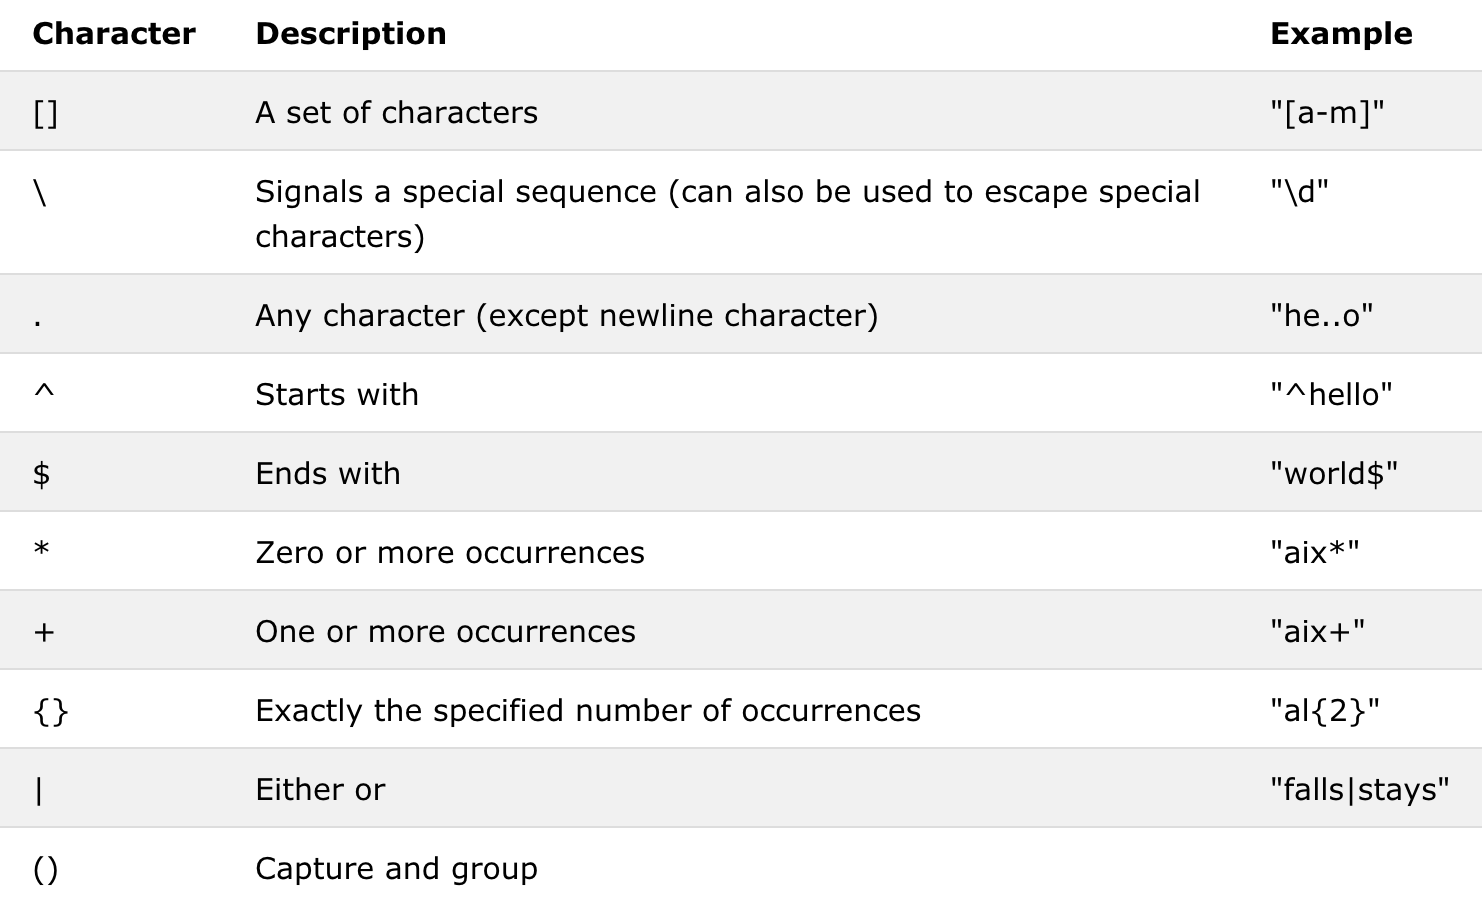
\includegraphics[scale=0.2]{regex.png}
		\caption{регулярные выражения в языке \\ программирования Python}
		\label{fig:regex}
	\end{figure}
	
	
	\subsection{Нормализация текста}
	
	Перед обработкой текста практически на любом естественном языке текст должен быть нормализован. Как минимум три задачи входят в любой процесс нормализации:
	
	1. Токенизация (сегментирование) слов
	
	2. Нормализация форматов слов
	
	3. Сегментирование предложений
	 
	В зависимости от приложения алгоритмы \textit{токенизации} могут токенизировать выражения из нескольких слов, такие как <<New York>> или <<Rock 'n' Roll>>, как один токен, для чего требуется некоторый словарь выражений из нескольких слов. Таким образом, токенизация тесно связана с обнаружением именованных объектов, задачей обнаружения имен, дат и	организации.
	
	Один широко используемый стандарт токенизации известен как стандарт токенизации \textit{Penn Treebank}, используемый для проанализированных корпусов (\textit{treebanks}), выпущена Linguistic Data Consortium (LDC), источником многих полезных наборов данных. Этот стандарт выделяет клитики, объединяет слова, написанные через дефисы, и выделяет все знаки препинания.
	На практике, поскольку токенизация должна выполняться перед любой другой языковой обработкой, она должна быть очень быстрой. Поэтому стандартный метод токенизации --
	использовать детерминированные алгоритмы, основанные на регулярных выражениях, скомпилированных в очень эффективные конечные автоматы.
	
	Токенизация в таких языках, как письменный китайский, японский и тайский, намного сложнее, так как они не используют пробелы для обозначения потенциальных границ слов.
	В китайском языке, например, слова состоят из символов (называемых ханзи). Каждый символ обычно представляет одну единицу значения (называется
	морфема) и произносится как один слог. Длина слов в среднем составляет около 2,4 символов. Но решить, что считать словом на китайском, сложно.
	
	
	Существует третий вариант токенизации текста. Вместо того, чтобы определять токены как слова
	или в виде символов (как на китайском), мы можем использовать данные для автоматического определения, какого размера токены должны быть. Возможно, иногда нам могут потребоваться токены -- разделенные пробелами
	слова; в других случаях полезно иметь токены размера больше, чем слова (например, New York Times), а иногда меньше, чем слова (например, морфема не-) Морфема - это наименьшая смысловая единица языка.
	
	\subsection{Byte Pair Encoding}
	
	Одна из причин, почему полезно иметь подслова в качестве токенов - когда есть неизвестные слова.
	Это особенно актуальны для систем машинного обучения. Они часто узнают некоторые факты о словах
	в одном корпусе (учебном), а затем используют эти факты для принятия решений в тестовом корпусе. Таким образом, если учебный корпус содержит, скажем,
	слова <<низкий>> и <<нижайший>>, но не <<ниже>>, но слово <<ниже>> появляется в тестовом
	корпусе, система не будет знать, что с этим делать.
	Решением этой проблемы является использование другого вида токенизации, в которой большинство токенов
	являются словами, но некоторые токены являются частыми морфемами или другими подсловами, такими как <<-ший>>, так что не появившееся в учебном корпусе слово может быть представлено путем объединения частей.
	
	Самый простой такой алгоритм -- это кодирование байтовой пары, или BPE (Byte Pair Encoging, также известный как Digram Coding \cite{5}).
	
	Алгоритм начинается с набора символов, равного набору букв в алфавите. Каждое	слово представлено в виде последовательности символов плюс специальный символ конца слова. На каждом шаге алгоритм подсчитывает количества пар букв, находит
	наиболее часто встречающуюся пару (A, B) и заменяет ее новым символом (AB). Алгоритм повторяется пока не произойдет $k$ слияний; $k$ является параметром алгоритма. Результирующий набор символов
	будет состоять из исходного набора букв плюс $k$ новых символов.
	Конечно, в реальных алгоритмах BPE выполняется со многими тысячами слияний на очень больших входных словарях. В результате большинство слов будет представлено как один символ и только очень редкие слова (и неизвестные слова) должны быть представлены по частям.
	
	\begin{figure}[H]
		\centering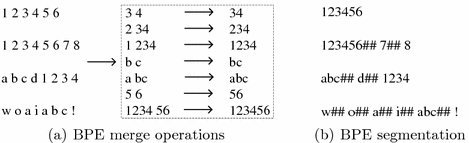
\includegraphics[scale=0.8]{bpe.png}
		\caption{пример выполнения алгоритма \\ BPE c 7 операциями слияния}
		\label{fig:bpe}
	\end{figure}
	
	
	\subsection{WordPiece}
	
	Есть несколько альтернатив алгоритму BPE. Как и BPE, алгоритм WordPiece начинается с некоторой простой токенизации (например, по пробелам), а затем разбивает получившиеся грубые лексемы на токены подслов. Модель WordPiece отличается от BPE тем, что специальные маркеры границ слова появляется в начале слова, а не в конце, и в том, как он объединяет пары. Вместо того, чтобы объединять наиболее часто встречающиеся пары, WordPiece объединяет те пары, которые максимизируют схожесть текста с выбранной языковой моделью на обучающей выборке. Тогда каждое слово токенизируется с использованием жадного алгоритма с самым длинным соответствием префиксу. Это отличается от алгоритма декодирования, который был введен для BPE, выполняющий слияния
	на тестовом тексте в том же порядке они были извлечены из учебного набора.
	Жадное декодирование с самым длинным соответствием префиксу иногда называют максимальным соответствием или максимальным паросочетанием.
	
	\subsection{Нормализация слов, лемматизация, стемминг}
	Нормализация слов -- это задание слов / токенов в стандартном формате, выбор одной нормальной формы для слов с несколькими формами.
	
	\textit{Сжатие регистра} -- переводит все слова в тексте в нижний регистр, это очень полезно для обобщения во многих задачах, таких как поиск информации или распознавание речь. Для анализа тональности текста и других задач классификации текста, извлечения информации и машинного перевода, напротив, регистр может оказаться весьма полезными и
	сжатие вообще не применяется.
	
	\textit{Лемматизация} определяет, имеют ли два слова имеют одинаковый корень,	несмотря на их поверхностные различия. Например, слова \textit{am}, \textit{are} и \textit{is} имеют общую лемму \textit{be}; 
	Самые сложные методы лемматизации предполагают полный морфологический анализ слова. (Морфология -- наука о том, как слова строятся из более мелких значащих единиц, называемых морфемами)
	
	
	Алгоритмы лемматизации могут быть достаточно сложными. По этой причине иногда используются более простые, но грубые методы, который в основном заключаются в обрезке аффиксов окончаний слова. Этот наивный вариант морфологического анализа называется \textit{стемминг}. Одним из наиболее распространенных алгоритмов стемминга является стеммирование Портера (1980). \cite{6}\\
	
	Стеммер Портера, примененный к следующему параграфу:
	
	\vspace{5mm}
	\begingroup
	\leftskip4em
	\rightskip\leftskip\textit{	This was not the map we found in Billy Bones's chest, but an accurate copy, complete in all things-names and heights and soundings-with the single exception of the red crosses and the written notes.}
	\vspace{5mm}
	\endgroup
	
	производит такой стеммированный вывод:
	
	\vspace{5mm}
	\begingroup
	\leftskip4em
	\rightskip\leftskip\textit{Thi wa not the map we found in Billi Bone s chest but an accur copi complet in all thing name and height and sound with the singl except of the red cross and the written note}
	\vspace{5mm}
	\endgroup
	
	
	\subsection{Расстояние Левенштейна}
	
	Расстояние Левенштейна \cite{7} или Minimum edit distance между двумя строками определяется как минимальное количество операций редактирования (такие операции, как: вставка, удаление,
	замена) необходимых для того, чтобы преобразовать одну строку в другую.
	Разрыв между \textit{intention} и \textit{execution}, например, равен 5 (удалить \textit{i}, заменить \textit{e} на \textit{n}, заменить \textit{x} на \textit{t}, вставить \textit{c}, заменить \textit{u} на \textit{n}). Это легче увидеть, посмотрев на Рисунок~\ref{fig:med}.
	
	
	\begin{figure}[H]
		\centering
\includegraphics[scale=0.8]{MED.PNG}
		\caption{Расстояние Левенштейна между словами "intention" и "execution". \\ Описание операций: d - удаление, s - замена, i - вставка.}
		\label{fig:med}
	\end{figure}
	
	\section{Языковые модели основанные на N-граммах.}
	Модели, которые сопоставляют последовательностям слов вероятности называются \textit{Language Models} (\textit{LM}, \textit{Языковые Модели}).
	
	\textit{N-грамма} -- это последовательность из N слов. 2-грамму называют \textit{биграммой} (\textit{bigram}), 3-грамму называют \textit{триграммой} (\textit{trigram}).
	В области обработки естественного языка N-граммы используется в основном для предугадывания на основе вероятностных моделей. N-граммная модель рассчитывает вероятность последнего слова N-граммы, если известны все предыдущие. При использовании этого подхода для моделирования языка предполагается, что появление каждого слова зависит только от предыдущих слов. \cite{8}
	
	Другим применением N-грамм является выявление плагиата. Если разделить текст на несколько небольших фрагментов, представленных N-граммами, их легко сравнить друг с другом и таким образом получить степень сходства анализируемых документов\cite{9}. N-граммы часто успешно используются для категоризации текста и языка. Кроме того, их можно использовать для создания функций, которые позволяют получать знания из текстовых данных. Используя N-граммы, можно эффективно найти кандидатов, чтобы заменить слова с ошибками правописания.
	
	\subsection{N-граммы}
	Рассмотрим задачу вычисления $P(w|h)$ -- вероятности, что следующим словом является $w$, при данной истории \textit{h}. Пусть история $h$: \textit{its water is so transparent that}, нужно узнать вероятность того, что следующим словом является \textit{the}, то есть, нужно найти:
	
	\begin{equation}
		\textit{P(the | its water is so transparent that)}
	\end{equation}
	
	Один из способов оценить эту вероятность -- по относительным частотам:	можно взять очень большой корпус, подсчитать, сколько раз встречается \textit{its water is so transparent that}, подсчитать, сколько раз за этим последует \textit{the}. Тогда это было бы ответом на вопрос "Мы видели историю h некоторое число раз, сколько раз следующее слово было \textit{the}":
	
	\begin{equation}
		\textit{P(the | its water is so transparent that) } = \dfrac{\textit{C(its water is so transparent that the)}}{\textit{C(its water is so transparent that)}}
	\end{equation}
	
	С огромным корпусом (например, Глобальная Сеть) можно рассчитать и посчитать вероятности с помощью формулы 1.1.
	
	Метод расчета вероятностей таким методом работает в многих случаях, но оказывается, что даже Глобальная Сеть недостаточно велика, чтобы дать хорошие оценки в большинстве случаев. Это происходит потому, что новые предложения создаются все время.
	
	Похожим образом, если нужно узнать вероятность появления какой-то последовательности из $n$ слов, нужно посчитать, сколько раз она появляется вреди всем последовательностей из $n$ слов. На это требуется огромная вычислительная сила.
	
	Есть способ умнее:
	обозначим вероятность того, что конкретное слово $X_i$ примет значение $w_i$ или $P(X_i)$ = $w_i$ за $P(w_i)$. Обозначим последовательность N слов как $w_1, w_2 \dots, w_n$ и как $w_1^n$. Обозначим совместную вероятность того, что каждое слова в последовательности имеет какое-то значение $P(X = w_1, Y = w_2, \dots, W = w_n)$ за $P(w_1, w_2, \dots, w_n)$. Теперь, чтобы вычислить вероятность целой последовательности $P(w_1, w_2, \dots, w_n)$ можно воспользоваться цепным правилом вероятностей: 
	
	\begin{equation}
	P(X_1, \dots, X_n) = P(X_1) P(X_2 | X_1) P(X_3 | X_1^2) \dots P(X_n | X_1^{n-1})
	\end{equation}
	 
	 Цепное правило показывает взаимосвязь между вычислением совместной вероятности последовательности и вычислением условной вероятности слова, при данных предыдущих словах. Формула 1.3 предполагает, что можно оценить совместную вероятность целой последовательности слов умножая между собой условные вероятности. Но похоже, что цепное правило не сильно-то и помогает, так как неизвестен способ вычисления точной вероятности слова после длинной последовательности предыдущих слов. $P(X_n | X_1^{n-1})$. Но с помощью N-грам можно аппроксимировать историю по нескольким предыдущим словам. 
	
	Биграмма, например, аппроксимирует вероятность слова по 1 предыдущему слову, то есть
	$P(w_n | w_1^{n-1}) \approx P(w_n | w_{n-1})$. 
	
	Предположение, что вероятность слова зависит только от предыдущего слова называется Марковым предположение. Марковские модели \cite{13} -- это класс вероятностных моделей, чтобы предполагают, что можно предсказать вероятность какого-то будущего события не смотря слишком далеко назад. Можно обобщить биграмму (которая смотрит только на одно слово в прошлое) до триграммы (которая смотрит на 2 слова в прошлое), а значит, по индукции, до N-граммы (которая смотрит на n-1 слово в прошлое).
	
	Таким образом, общее уравнение для этой N-граммной аппроксимации условной вероятности следующего слова в предложении таково:
	
	\begin{equation}
	 P(w_n | w_1^{n-1}) \approx P(w_n | w_{n+1-N}^{n-1}) 
	\end{equation}
	 
	 При заданном биграмном предположении для вероятности отдельного слова, можно вычислить вероятность полной последовательности слов:
	 
	\begin{equation}
		P(w_1^n) \approx \prod_{k=1}^{n} P(w_k | w_{k-1})
	\end{equation}
	
	Для того, чтобы оценить вероятности этих биграм или n-грам можно использовать \textit{метод наибольшего правдоподобия} (\textit{maximum likelihood estimation}, \textit{MLE}). 
	
	Мы получаем оценки MLE для параметров N-граммы подсчитав их в корпусе и нормализовав их таким образом, чтобы они лежали между 0 и 1.
	
	Например, чтобы вычислить конкретную биграммную вероятность слова $y$ при предыдущем слова $x$, нужно вычислить количество биграмм $C(xy)$ и нормализовать по сумма всех биграмм, у которых первое слово $x$.
	
	\begin{equation}
		P(w_n | w_{n-1}) = \dfrac{C(w_{n-1}w_n)}{\sum_w C(w_{n-1}w)}
	\end{equation}
	
	Формулу 1.6 можно упростить, заметив, что количество биграмм, начинающихся с $w_{n-1}$ должно быть равно количество слов $w_{n-1}$. 
	
	\begin{equation}
		P(w_n | w_{n-1}) = \dfrac{C(w_{n-1}w_n)}{C(w_{n-1})}
	\end{equation}


	Для общего случая MLE, оценка параметра n-граммы:
	
	
	\begin{equation}
		P(w_n | w_{n-N+1}^{n-1}) = \dfrac{C(w_{n-N+1}^{n-1} w_n)}{C(w_{n-N+1}^{n-1})}
	\end{equation}
	
	Формула 1.8 оценивает вероятность N-граммы деля увиденную частоту конкретной последовательности на увиденную частоту префикса. Это отношение называется \textit{относительной частотой}.
	
	В практике применяются триграммы, 4-граммы или даже 5-граммы, в зависимости от объема обучающей выборки. 
	
	Также, чаще всего используются \textit{логарифмические вероятности}, так как перемножение большого числа вероятностей может дать слишком маленькое число, которое может "сломать" разрядную сетку вещественного числа в цифровом представлении. При использовании логарифмов умножение заменяется на сложение, следовательно, число не будет слишком мало.
	
	
	\begin{equation}
		p_1 \times p_2 \times p_3 \times p_4 = exp(log(p_1) + log(p_2) + log(p_3) + log(p_4))
	\end{equation}
	
	\subsection{Оценка языковых моделей}
	Лучший способ оценить производительность языковой модели - это непосредственно встроить её в систему и вычислить, насколько система улучшается. Такой подход называется \textit{внешней оценкой}. Внешняя оценка -- это единственный способ узнать, помогает ли в решении задачи конкретное улучшение какой-то компоненты. Таким образом, для распознавания речи можно сравнить производительность двух языковых моделей, запустив дважды распознаватель и посмотреть, какой запуск дает более точный перевод.
	
	К сожалению, запуск больших NLP систем от начала до конца - это очень дорого. Вместо этого хорошо бы иметь метрику, которая может дать быструю оценку потенциального улучшения в языковой модели. Метрика \textit{внутренней оценки} - это одна из мер качества модели, вне зависимости от приложения. 
	
	Для внутренней оценки языковой модели требуется \textit{тестовая выборка}. Как и с многими другими статистическими моделями, вероятности N-граммовой модели выходят из корпуса, на котором модель обучалась, которая называется \textit{обучающей выборкой}. После этого можно оценить качество модели на основе её производительности на каких-то еще неиспользованных данных, которые и называются \textit{тестовой выборкой}.
	
	Если задан какой-то корпус текста, он делится на обучающую и тестовую выборки, после этого обучаются на обучающей и проверяются на тестовой. Потом происходит сравнение двух обученных моделей: насколько хорошо они удовлетворяют тестовой выборке.
	
	Очень важно не допустить того, чтобы информация из тестовой выборки встречалась в обучающей. Если это происходит, попавшему туда предложению ошибочно ставится большая вероятность. Это называют \textit{обучением на тестовой выборке}. 
	
	Иногда тестовая выборка используется настолько часто, что модель явным образом подгоняется под её характеристики. Для того, чтобы этого избежать, используют свежие данные, не использованные ни в тестовой, ни в обучающей выборке. Эти данные называют \textit{валидационной выборкой} (\textit{development test set}, \textit{devset}). 
	
	\subsection{Перплексия}
	На практике, вероятности не используются для метрики оценки языковой модели. Вместо этого используется \textit{перплексия} (иногда называют \textit{PP}). Перплексия языковой модели на тестовой выборке - это обратная величина к вероятности на тестовой выборке, нормализованная количеством слов. Для тестовой выборки $W = w_1 w_2 \dots w_N$ :
	
	\begin{equation}
		PP(W) = P(w_1 w_2 \dots w_n)^{-\frac{1}{N}}
	\end{equation}
	
	Можно использовать цепное правило, чтобы раскрыть вероятность W:
	
	\begin{equation}
		PP(W) = (\prod_{i=1}^{N} \frac{1}{P(w_i | w_1 \dots w_{i-1})})^{\frac{-1}{N}}
	\end{equation}
	
	Если вычислять перплексию с помощью биграммной языковой модели:
	
	
	\begin{equation}
		PP(W) = (\prod_{i=1}^{N} \frac{1}{P(w_i | w_{i-1})})^{\frac{-1}{N}}
	\end{equation}
	
	Можно представить перплексию по-другому, \textit{как взвешенное среднее количество сыновей вершины графа}. Количество сыновей - это количество различных слов, которые могут последовать за текущим.
	
	\subsection{Неизвестные слова}
	Неизвестные слова не могут появиться в тестовой выборке, если используется \textit{закрытый словарь}, который содержит все слова в лексиконе. В других случаях придется обрабатывать слова, никогда ранее не встречавшиеся, назовем такие слова \textit{неизвестными} или \textit{словами вне словаря} (\textit{out of vocabulary}, \textit{OOV}). Процент неизвестных слов, которые попадаются в тестовой выборке, называют \textit{мерой неизвестности} (\textit{OOV rate}). Система с \textit{открытым словарем} - в которой неизвестные слова добавляются как псевдо-слово <UNK>.
	
	Есть несколько способов обучить вероятности слов <UNK>. Один из них - это свести задачу назад к закрытому словарю, добавив слово <UNK> в словарь на стадии нормализации текста, после этого обращаясь к нему как к любому другому слову.
	
	\subsection{Сглаживание}
	Самый простой способ - это просто добавить один ко всем количествам биграмм перед тем, как производить нормализацию их в вероятности. Этот алгоритм называется \textit{сглаживанием Лапласа}. Оно недостаточно хорошо себя показывает, чтобы использовать его в современных моделях на N-граммах, но дает множество полезных идей, которые используются в других алгоритмах сжатия, также является практичным алгоритмам для таких задач, как \textit{классификация текста}.
	
	Оценка вероятности появления слова $w_i$ - это его количество $с_i$, нормализованное общим числом слов $N$.
	
	\begin{equation}
		P(w_i) = \dfrac{c_i}{N}
	\end{equation}
	
	Сглаживание Лапласа добавляет 1 ко всем количествам. Всего есть $V$ уникальных слов в словаре, к каждому добавляется 1, значит знаменатель увеличивается на $V$.
	
	\begin{equation}
		P_{Laplace}(w_i) = \dfrac{c_i + 1}{N + V}
	\end{equation}
	
	
	Сглаживание для вероятностей биграмм:
	
	\begin{equation}
		P^{*}_{Laplace}(w_n | w_{n-1}) = \dfrac{C(w_{n-1} w_n) + 1}{\sum_w (C(w_{n-1} w) + 1)} = \dfrac{C(w_{n-1} w_n) + 1}{C(w_{n-1}) + V}
	\end{equation}
	
	Альтернативный способ сглаживания - прибавлять ко всем количествам не 1, а k. Этот алгоритм называется \textit{<<прибавь k>>-сглаживание} (\textit{add-k smoothing}).
	
	\begin{equation}
		P^{*}_{Add-k}(w_n | w_{n-1}) = \dfrac{C(w_{n-1} w_n) + k}{\sum_w (C(w_{n-1} w) + k)} = \dfrac{C(w_{n-1} w_n) + 1}{C(w_{n-1}) + kV}
	\end{equation}
	 
	 \subsection{Интерполяция}
	 
	 Иногда, когда требуется вычислить $P(w_n | w_{n-1})$, но нет примера триграммы $w_{n-2}w_{n-1}w_{n}$, можно оценить вероятность используя биграммную вероятность $P(w_{n} | w_{n-1})$. Похожим образом, если нет примеров биграммы $P(w_n | w_{n-1})$, можно воспользоваться $P(w_n)$.
	 
	 Примером такого использования является \textit{интерполяция}, она вычисляет оценку вероятности взвешивая и комбинируя триграмму, биграмму и юниграмму.
	 
	 В простой линейной интерполяции оценки комбинируются линейно:
	 
	 \begin{equation}
	 	P^{'}(w_n | w_{n-2} w_{n-1}) = \lambda_1 P(w_n | w_{n-2} w_{n-1}) + \lambda_2 P(w_n | w_{n-2}) + \lambda_3 P(w_n)
	 \end{equation}
	 
	 
	 \begin{equation}
	 	\sum_i \lambda_i = 1
	 \end{equation}
	 
	 Способ сложнее - давать каждой $\lambda$ вес, зависящий от контекста. Если имеются точное количество для какой-то биграммы, можно сделать предположение, что число триграмм, основанных на этой биграмме будет заслуживать большего доверия, а значит можно дать соответствующей $\lambda$ больший вес:
	 
	 \begin{equation}
	 	P^{'}(w_n | w_{n-2} w_{n-1}) = \lambda_1 (w_{n-2}^{n-1}) P(w_n | w_{n-2} w_{n-1}) + \lambda_2 (w_{n-2}^{n-1}) P(w_n | w_{n-2}) + \lambda_3 (w_{n-2}^{n-1}) P(w_n)
	 \end{equation}
	 
	  Для того, чтобы вычислить все $\lambda_i$, пользуются \textit{сохранённым} (\textit{held-out}) корпусом - дополнительным обучающей выборкой, которую используют для настройки параметров системы, таких, как $\lambda$. 
	
	\section{Подходы и методы, основанные на наивном Байесе.}
	
	\textit{Наивный Байес} зачастую применяется к задаче \textit{категоризации текста} - присваиванию категории к целым текстам или документам, например, к \textit{анализу тональности текста}, то есть выделению, например, положительного или отрицательного настроя автора к какому-либо объекту. \cite{14}
	
	 \textit{Обнаружение спама} - еще одно приложение. Задача бинарной классификации, состоящая в том, чтобы дать электронному письму оценку, является ли оно спамом.
	 
	 Цель классификации состоит в том, чтобы произвести простые наблюдения, выделить какие-либо полезные черты и классифицировать наблюдения в какой-то дискретный класс.
	 
	 \subsection{Наивный Байес}
	 
	 Интуитивное описание показано на рисунке~\ref{fig:NaiveBayes}. Текст представляется как \textit{мешок слов}, то есть неупорядоченное множество слов, их взамное расположение проигнорировано, сохранены только частоты появления слова в тексте.
	 
	 
	 \begin{figure}[H]
	 	\centering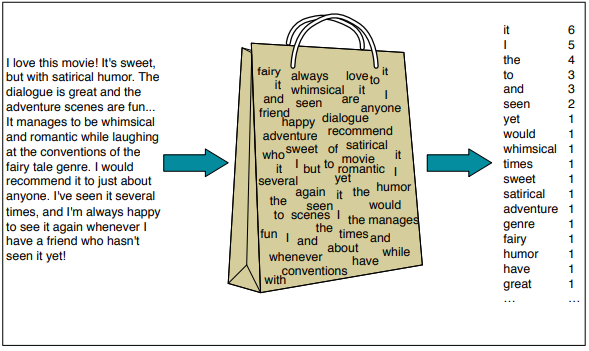
\includegraphics[scale=0.9]{NaiveBayes.PNG}
	 	\caption{Интуитивное описание классификатора на наивном Байесе, применённое к обзору фильма. Взаимное расположение слов игнорировано (взято предположение \textit{мешка слов}).}
	 	\label{fig:NaiveBayes}
	 \end{figure}
	  
	  Наивный Байес - это вероятностный классификатор, означающий, что для документа $d$ из всех классов $c \in C$ классификатор возвращает класс $\hat{c}$ который имеет максимальную вероятность встречи в тексте. В формуле 1.20 нотация $\hat{}$ означает предполагаемый корректный класс. 
	
	\begin{equation}
		\hat{c} = \underset{c \in C}{argmax} P(c | d)
	\end{equation}
	
	Эта идея \textit{Байесовского вывода} была известна с момента публикации работы Байеса (1763) \cite{10}, и была впервые применена к классификации текста Мостеллером и Уоллесом (1964) \cite{11}. Идея Байесовского классификатора - использовать правило Байеса и трансформировать предыдущее уравнение в другие вероятности, имеющие полезные свойства. Правило Байеса представлено в следующем уравнении. Оно дает способ разбить условную вероятность $P(x | y)$ в три другие вероятности:
	
	
	\begin{equation}
		P(x | y) = \dfrac{P(y | x) P(x)}{P(y)}
	\end{equation}
	
	Используя  формулу 1.20.
	
	\begin{equation}
		\hat{c} = \underset{c \in C}{argmax} P(c | d) = \underset{c \in C}{argmax} \dfrac{P(d | c) P(c)}{P(d)}
	\end{equation}
	
	Знаменатель можно опустить.
	
	\begin{equation}
		\hat{c} = \underset{c \in C}{argmax} P(c | d) = \underset{c \in C}{argmax} P(d | c) P(c)
	\end{equation}

	Таким образом вычисляется самый вероятный класс $\hat{c}$ по заданному документу $d$ с помощью класса который имеет наибольшее произведение двух вероятностей: априорная вероятность класса $P(c)$ и функция правдоподобия документа  $P(d | c)$.
	
	
	\begin{equation}
		\hat{c} = \underset{c \in C}{argmax} P(c | d) = \underset{c \in C}{argmax} \overset{likelihood}{P(d | c)} \overset{prior}{P(c)}
	\end{equation}
	
	Не умаляя общности, можно представить документ $d$ как набор черт $f_1, f_2, \dots, f_n$.
	
	
	\begin{equation}
		\hat{c} = \underset{c \in C}{argmax} \overset{likelihood}{P(f_1, f_2, \dots, f_n | c)} \overset{prior}{P(c)}
	\end{equation}
	
	
	К сожалению, даже формула 1.25 тяжела для вычисления: без какиих-либо упрощающих предположений оценка вероятность любой возможной комбинации черт потребует огромного числа параметров и невозможно большую обучающую выборку. Поэтому Наивный Байес делает два упрощающих предположения.
	
	Первое - это \textit{мешок слов} (\textit{bag of words}): предположение, что позиция слова не имеет значения. Например, слово \textit{любовь} будет иметь один и тот же эффект вне зависимости от того, чтоит оно на первом, двадцатом или последнем месте в тексте.
	
	Второе часто называют \textit{предположением наивного Байеса}:
	это предположение условной независимости того, что вероятности $P(f_i | c)$ независимы при данном классе $c$ и могут быть <<наивно>> перемножены таким способом:
	
	\begin{equation}
		P(f_i, f_2, \dots f_n | c) = P(f_1 | c) P(f_2 | c) \dots P(f_n | c)
	\end{equation}
	
	Результирующее уравнение для класса выбранного наивным Байесом таково:
	
	\begin{equation}
		C_{NB} = \underset{c \in C}{argmax} P(c) \underset{f \in F}{\prod} P(f | c)
	\end{equation}
	
	Для того, чтобы применить наивного Байеса к тексту, нужно учесть позиции, просто проверяя индексом каждую позицию слова в документе:
	
	\begin{center}
	positions $\leftarrow$ все позиции слов в тестовом документе
	\end{center}
	\begin{equation}	
	C_{NB} = \underset{c \in C}{argmax} P(c) \underset{i \in positions}{\prod} P(w_i | c)
	\end{equation}
	
	 
	 \subsection{Наивный Байес как лингвистическая модель}
	 
	 Байесовские классификаторы могут использовать любые виды черт: словари, URL, e-mail адреса, черты сети, фразы и тому подобное. Но если, как в предыдущей секции, используются только черты отдельных слов и используются все слова в тексте, то наивный Байес имеет важную схожесть с моделированием речи. Конкретнее, модели на наивном Байесе могут быть рассмотрены как множество классо-специфичных юниграммных лингвистических моделей.
	 
	 Поскольку  правдоподобие черт из модели наивного Байеса присваивает вероятность для каждого слова $P(word | c)$, модель также присваивает вероятность целым предложениям.
	 
	 \begin{equation}
	 	P(s | c) = \prod_{i \in positions} P(w_i | c) 
	 \end{equation}
	 
	 \subsection{Метрики: точность, полнота, F-мера}
	 
	 Рассмотрим задачу обнаружения спама. Задача состоит в том, чтобы отнести каждое электронное письмо к одной из двух категорий: положительной (то есть, является спамом) или отрицательной (то есть, не является). Таким образом, для каждого письма требуется узнать, считает ли система его спамом или нет. Также требуется знать, является ли письмо спамом на самом деле, то есть определенные человеком ярлыки для каждого письма.Таким метки будут далее называться \textit{золотыми ярлыками} (\textit{gold labels}).
	 
	 Для оценки любой системы распознавания требуется начать с постройки \textit{таблицы сопряженности}.
	 
	 \begin{figure}[H]
	 	\centering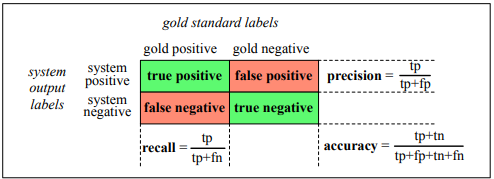
\includegraphics[scale=0.9]{conttable.PNG}
	 	\caption{таблица сопряженности}
	 	\label{fig:conttable}
	 \end{figure}
	 
	 В правом нижнем углу таблицы уравнение для \textit{accuracy}, которое показывает какую часть всех наблюдений система обозначила правильно. Хотя accuracy может показаться вполне естественной метрикой, она используется нечасто. Причина заключается в том, что accuracy работает плохо, если классы не сбалансированы. Другими словами, accuracy плоха, если требуется найти что-то редко встречающееся, или по крайней мере просто не сбалансировано по частоте встречи. 
	 
	 Именно поэтому вместо accuracy используются 2 метрики: \textit{полнота} и \textit{точность} (\textit{precision} и \textit{recall}).
	 
	 \textit{Точность} обозначает долю прецедентов которые система система обозначила как положительные и которые на самом деле являются положительными (то есть, например, обозначила как спам и письмо действительно им является).
	 
	 \begin{equation}
    	Precision = \dfrac{\textit{true positives}}{\textit{true positioves + false positives}}
	 \end{equation}
	 
	 \textit{Полнота} обозначает долю прецедентов, которые были корректно обозначены положительными (то есть среди всех писем обозначенных как спам доля тех, которые действительно им являлись).
	 
	 \begin{equation}
	 Precision = \dfrac{\textit{true positives}}{\textit{true positioves + false negatives}}
	 \end{equation}
	 
	 Есть много способов определения единой метрики, которая сочетает в себе оба аспекта полноты и точности. Самая простая из этих комбинаций: \textit{F-мера}.
	 
	 \begin{equation}
	 F_\beta = \dfrac{(\beta^2 + 1) P R}{\beta^2 P + R} 
	 \end{equation}
	 
	 Параметр $\beta$ взвешивает важность полноты и точности, его задают в зависимости от задачи. Значения $\beta$ > 1 отдают предпочтение точности, $\beta$ < 1 - полноте. Когда $\beta$ = 1, метрики равно сбалансированы; это самый частый случай использования, обозначается $F_{\beta = 1}$ или $F_1$: 
	 
	 \begin{equation}
	 F_1 = \dfrac{2PR}{P + R}
	 \end{equation}
	 
	 
	 Для случая, когда есть больше, чем 2 класса.
	 В обработке языка часто встречается \textit{мультиномиальная классификация}, в который классы - взаимоисключающие, каждый документ относится к одному классу. Для каждого класса строится свой бинарный классификатор, обучающийся на положительных результатах из класса \textit{c} и отрицательных из всех остальных классов. После этого заданный документ \textit{d} обрабатывается всеми классификаторами и выбирается ярлык из классификатора с наивысшим результатом. Рассмотрим \textit{матрицу ошибок} для гипотетической категоризации писем по классам \textit{важные}, \textit{обычные}, \textit{спам} (\textit{urgent}, \textit{normal}, \textit{spam}).
	 
	 \begin{figure}[H]
	 	\centering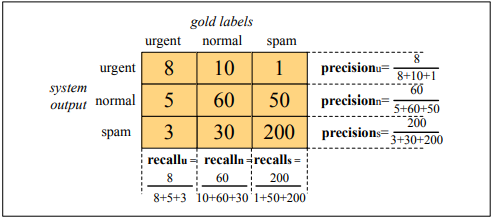
\includegraphics[scale=0.9]{confmatrix.PNG}
	 	\caption{матрица ошибок (confusion matrix)}
	 	\label{fig:confmatrix}
	 \end{figure}
	
	Для того, чтобы выделить единую метрику для производительности системы в целом, можно воспользоваться \textit{макроусреднением} (\textit{macroaveraging}) или \textit{микроусреднением} (\textit{microaveraging}).
	
	\textit{Макроусреднение} - это вычисление производительности для каждого класса, а потом взятие среднего.
	\textit{Микроусреднение} - это сбор всех решений в единую таблицу сопряженности и вычисление полноты и точности по ней. На рисунке~\ref{fig:micromacro} показана разница между этими двумя способами. 
	
	\begin{figure}[H]
		\centering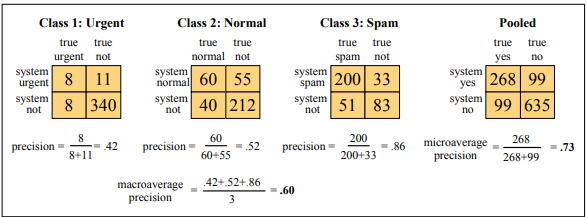
\includegraphics[scale=0.9]{micromacro.PNG}
		\caption{макроусреднение и микроусреднение}
		\label{fig:micromacro}
	\end{figure}
	
	
	\subsection{Тестовые выборки и кросс-валидация}
	С фиксированными выборками возникает следующая проблема: так как для обучающей выборки нужно как можно больше прецедентов, тестовая или валидационная выборка могут оказаться недостаточно большими, чтобы быть репрезентативными. Лучшим вариантом было бы, если можно было бы использовать всю информацию а одновременно тестовой и обучающей выборке. Это позволяет сделать \textit{кросс-валидация} \cite{15} :
	случайным образом весь датасет разбивается на обучающую и тестовую выборки, классификатор обучается и проверяется на разбитых множествах. 
	Эта процедура происходит 10 раз, средний результат среди 10 попыток дает оценку ошибок. Всё это называется \textit{10-слойной кросс-валидацией}.
	

	\section{Вероятностные тематические модели}
	
	Базовые вероятностные тематические модели \cite{22} (probabilistic topic model) основаны на следующих предположениях:
	
	\begin{itemize}
		\item порядок документов в коллекции не важен;
		\item порядок слов в документе не важен;
		\item слова, встречающиеся в большинстве документов, не важны для определения тематики, их обычно исключают из словаря и называют стоп-словами;
		\item слово в разных формах — это одно и то же слово;
		\item коллекцию документов можно рассматривать как простую выборку пар «документ–слово» $(d, w), d \in D, w \in W_d$;
		\item каждая тема $t \in T$ описывается неизвестным распределением $p(w | t)$ на множестве слов $w \in W$
		\item каждый документ $d \in D$ описывается неизвестным распределением $p(t|d)$ на множестве тем $t \in T$;
		\item гипотеза условной независимости: $p(w|t,d)=p(w|t)$.
	\end{itemize}
	
	Построить тематическую модель — значит, найти матрицы $\Phi = ||p(w|t)||$ и $\Theta = ||p(t|d)||$ по коллекции $D$.
	
	В более сложных вероятностных тематических моделях некоторые из этих предположений заменяются более реалистичными. Например, вместо модели «мешка слов» может использоваться марковская цепь; множество документов может рассматриваться как упорядоченное по времени их создания, и т. д.
	
	
	\subsection{Вероятностный латентный семантический анализ}
	
	Вероятностный латентный семантический анализ (probabilistic latent semantic analysis, PLSA) предложен Томасом Хофманном в 1999 году.
	
	Вероятностная модель появления пары «документ–слово» $(d,w)$ может быть записана тремя эквивалентными способами:
	
	$p(d,w) = \sum_{t\in T} p(t) p(w|t) p(d|t) = \sum_{t\in T} p(d) p(w|t) p(t|d) = \sum_{t\in T} p(w) p(t|w) p(d|t)$,
	где $T$ — множество тем;
	
	$p(t)$ — неизвестное априорное распределение тем во всей коллекции;
	$p(d)$ — априорное распределение на множестве документов, эмпирическая оценка $p(d)$ = $n_d/n$, где $n = \sum_d n_d$ — суммарная длина всех документов;
	$p(w)$ — априорное распределение на множестве слов, эмпирическая оценка $p(w) = n_w/n$, где $n_w$ — число вхождений слова w во все документы;
	Искомые условные распределения $ p(w|t),\: p(t|d) $ выражаются через $ p(t|w),\: p(d|t) $ по формуле Байеса:
	
	\begin{equation}
	p(w|t) = \frac{p(t|w)p(w)}{\sum_{w'} p(t|w')p(w')};\qquad  p(t|d) = \frac{p(d|t)p(t)}{\sum_{t'} p(d|t')p(t')}.
	\end{equation}
	
	Для идентификации параметров тематической модели по коллекции документов применяется принцип максимума правдоподобия, который приводит к задаче максимизации функционала
	
	\begin{equation}
	\sum_{d\in D} \sum_{w\in d} n_{dw}\log p(w|d) \to \max_{\Phi,\Theta} ,
	\end{equation}
	при ограничениях нормировки
	
	\begin{equation}
	\sum_w p(w|t) = 1,\; \sum_t p(t|d) = 1,\; \sum_t p(t) = 1,
	\end{equation}
	где $n_{dw}$ — число вхождений слова w в документ d.
	
	Для решения данной оптимизационной задачи обычно применяется EM-алгоритм.
	
	Основные недостатки PLSA:
	
	\begin{itemize}
	\item Число параметров растёт линейно по числу документов в коллекции, что может приводить к переобучению модели.
	\item При добавлении нового документа d в коллекцию распределение $p(t|d)$ невозможно вычислить по тем же формулам, что и для остальных документов, не перестраивая всю модель заново.
	\end{itemize}
	
	
	
	\subsection{Латентное размещение Дирихле}
	
	Метод латентного размещения Дирихле \cite{21} (latent Dirichlet allocation, LDA) предложен Дэвидом Блеем в 2003 году. В этом методе устранены основные недостатки PLSA.
	
	Метод LDA основан на той же вероятностной модели
	
	\begin{equation}
	p(d,w) = \sum_{t\in T} p(d) p(w|t) p(t|d),
	\end{equation}
	при дополнительных предположениях:
	
	\begin{itemize}
	\item векторы документов $\theta_d = \bigl(p(t|d):\: t\in T\bigr)$ порождаются одним и тем же вероятностным распределением на нормированных |T|-мерных векторах; это распределение удобно взять из параметрического семейства распределений Дирихле $\mathrm{Dir}(\theta,\alpha),\; \alpha\in\mathbb{R}^{|T|};$
	\item векторы тем $\phi_t = \bigl(p(w|t):\: w\in W\bigr)$ порождаются одним и тем же вероятностным распределением на нормированных векторах размерности |W|; это распределение удобно взять из параметрического семейства распределений Дирихле $\mathrm{Dir}(\theta,\beta),\; \beta\in\mathbb{R}^{|W|}$.
	
\end{itemize}
	
	Для идентификации параметров модели LDA по коллекции документов применяется самплирование Гиббса, вариационный байесовский вывод или метод Expectation-Propagation.
	
	
	
	
	
	\subsection{Распределение Дирихле}
	Распределение Дирихле \cite{20} -- непрерывное распределение вероятностей, носителем которого является $k$-мерный симплекс ($k$-мерный тетраэдр):
	
	\begin{equation}
	\Delta_k = \{q \in \mathbb{R} | \sum_{i=1}^k q_i = 1, q_j \geq 0, j = 0, \dots, k\}.
	\end{equation}
	
	Плотность вероятности распределения Дирихле задаётся следующей формулой:
	
	\begin{equation}
	Dir(q | \alpha) = \frac{\Gamma (\sum_{i=1}^k \alpha_i)}{\Pi_{i=1}^k \Gamma(\alpha_i)} \Pi_{i=1}^k q_i^{a_i - 1}, q \in \Delta_k
	\end{equation}
	
	где $\alpha = (\alpha_i)_{i=1}^k, a_i > 0$ -- вектор параметров распределения, $\Gamma(\dots)$ -- гамма функция. Графики плотности распределения Дирихле при различных значениях параметров приведены на рисунке~\ref{fig:derihlet}
	
	\begin{figure}[H]
		\centering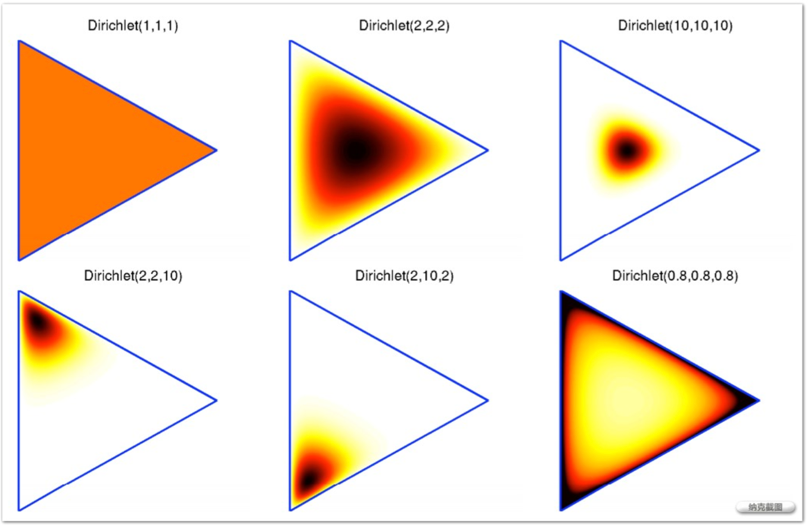
\includegraphics[scale=0.8]{derihlet.PNG}
		\caption{Различные виды плотности распределения Дирихле при $k = 3$}
		\label{fig:derihlet}
	\end{figure}
	
	
	\textbf{Связь с бета-распредлением.} В случае $k = 2$ распределение Дирихле тесно связано с бета-распределением:
	
	\begin{equation}
	Beta(x | \alpha, \beta) = \frac{\Gamma(\alpha + \beta)}{\Gamma(\alpha) \Gamma(\beta)} x^{\alpha - 1} (1-x)^{\beta - 1}, 0 \leq x \leq 1
	\end{equation}
	
	\textbf{Связь с мультиномиальным распределением.} Распределение Дирихле является сопряженным к мультиномиальному распределению:
	
	\begin{equation}
	Mult(x | k, n, x) = \frac{n!}{x_1! \dots x_k!} \Pi_{i=1}^k q_i^{x_i}, x_i = 0, \dots, n, i = 1, \dots, k, \sum_{i=1}^k x_i = n,
	\end{equation}
	
	где $n \in \mathbb{N}, k \in \mathbb{N}, q \in \Delta_k$ - параметры распределения, $n$ - общее число испытаний, $k$ - количество возможных исходов каждого из испытаний, $q$ - вектор вероятностей выпадения каждого из исходов в каждом испытании.
	
	
		
		
	\section{Логистическая регрессия}	
	\textit{Логистическая регрессия} - один из самых важных аналитических инструментов в социальных и естественных науках. В обработке естественного языка логистическая регрессия - базовый метод машинного обучения с учителем для классификации. Имеет очень близкое отношение к нейронным сетям \cite{18}. 
	Логистическая регрессия используется, чтобы классифицировать наблюдения в одни из 2 или более классов. Так как математика под двухклассовым случаем проще, сначала будет описана именно она. Затем будет описан случай мультиномиальной логистической регрессии для случая большего числа классов. 
	
	\subsection{Генеративные и дискриминативные классификаторы}.
	
	Самое важное отличие наивного Байеса от логистической регрессии состоит в том, что логистическая регрессия - \textit{дискриминативный классификатор}, а наивный Байес - \textit{генеративный}. Можно рассмотреть на визуальной метафоре: пусть задачей является отделить картинки кошек от собак. 
	
	\textit{Генеративный} классификатор будет иметь цель понять как выглядит кошка и собака. Можно даже заставить модель <<сгенерировать>>, то есть нарисовать собаку. При подаче тестового изображения система спрашивает, какая модель - кошки или собаки лучше подходит под изображение и, отталкиваясь от этого, выбирает ярлык.
	
	\textit{Дискриминативная} модель учится именно разделять классы. Возможно, все собаки носят ошейники, а все кошки - не носят. Если эта черта почти полностью разделяет классы, модели этого достаточно. Если спросить модель, что она знает о кошках, она ответит, что они не носят ошейников.
	
	Генеративная модель, такая, как наивный Байес, использует термин \textit{правдоподобие}, который выражает, как генерировать черты документа, если бы мы знали какого он класса.
	
	Дискриминативная модель пытается непосредственно вычислить $P(c | d)$. Похоже, что она учится присваивать веса к чертам документа, которые непосредственно улучшают способность разделять между классами, даже если модель не может сгенерировать пример одного из классов.
	
	
	\subsection{Компоненты вероятностного классификатора для машинного обучения}
	Как и наивный Байес, логистическая регрессия - это вероятностный классификатор, использующий \textit{обучение с учителем}. Классификаторы машинного обучения требуют корпус из M пар ввода-вывода ($x^{(i)}$, $y^{(i)}$).
	
	Система машинного обучения для классификации имеет 4 компоненты:
	\begin{enumerate}
		\item Репрезентация черт ввода. Для каждого наблюдения $x^{(i)}$ это вектор черт $[x_1, x_2, \dots, x_n]$. Обозначение: черта \textit{i} прецедента $x^{(j)}$ это $x_i^{(j)}$, иногда упрощенно $x_i$, иногда $f_i$, $f_i(x)$, или, для мультиклассовой классификации, $f_i(c, x)$.
		
		\item Функция классификации, которая вычисляет $\hat{y}$, предполагаемый класс, как $p(y | x)$. В следующей секции будут введены инструменты \textit{сигмоида} \cite{16} и \textit{софтмакс} для классификации. 
		
		\item Целевая функция для обучения, обычно включающая минимизацию ошибки на обучающей выборке. 
		
		\item Алгоритм для оптимизации целевой функции. Далее в работе будет представлен \textit{алгоритм стохастического градиентного спуска}.		
		
	\end{enumerate}
	
	
	Логистическая регрессия имеет 2 фазы:
	\begin{enumerate}
		\item обучение: система учится (а именно веса $w$ и $b$), используя стохастический градиентный спуск и функцию потерь \textit{кросс-энтропии}.
		
		\item проверка: по заданному прецеденту $x$ вычисляется $P(y | x)$ и возвращается большая вероятность: $y = 1$ или $y = 0$.
		
	\end{enumerate}
	
	
	\subsection{Классификация: сигмоида}
	
	Целью бинарной логистической регрессии является обучение классификатора таким образом, чтобы он мог давать бинарное предсказание о классе нового прецедента. Здесь будет описана \textit{сигмоида}, помогающая принять такое решение.
	
	Рассмотрим единственный прецедент $x$, который будет обозначаться как вектор черт $[x_1, x_2, \dots, x_n]$. Вывод классификатора может $y$ может быть равен 1 (это означает, что прецедент является членом класса) или 0 (не является). Требуется узнать вероятность $P(y = 1 | x)$ того, что прецедент является членом класса.
	
	Логистическая регрессия добивается этого, обучая на выборке вектор весов и меру смещения. Каждый вес $w_i$ - действительное число, ассоциировано с чертой $x_i$. Вес обозначает, насколько важна эта черта для классификации определенного класса, вес может быть положительным (значит, что ассоциировано) или отрицательным (не связано). 
	
	Чтобы сделать решение на тестовом случае, после того, как веса обучены, классификатор умножает каждый $x_i$ на его вес $w_i$ и прибавляет меру смещения $b$. Результирующее число $z$ обозначает взвешенную сумму всех всидетельств класса.
	
	\begin{equation}
	z = (\sum_{i=1}^n w_i x_i) + b
	\end{equation}
	
	Можно записать это уравнение короче, если воспользоваться скалярным произведением:
	
	\begin{equation}
	z = w \cdot x + b
	\end{equation}
	
	
	В предыдущем уравнении ничего не останавливает $z$ от того, чтобы перестать быть валидной вероятностью, то есть выйти из границ $[0, 1]$.  
	
	\begin{figure}[H]
		\centering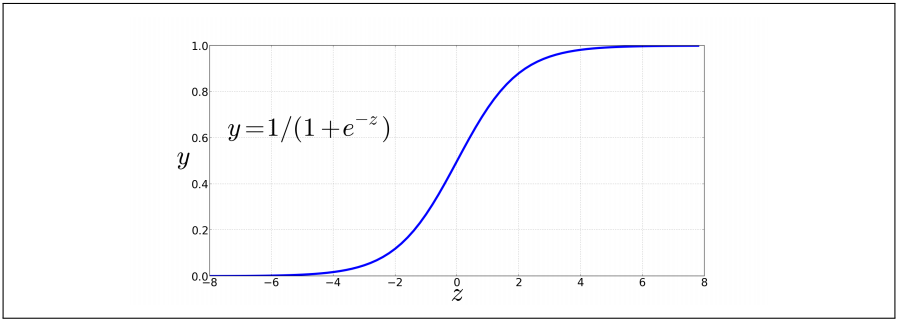
\includegraphics[scale=0.8]{sigmoid.PNG}
		\caption{сигмоида, на вход получает действительное число, на выходе - число из интервала $[0, 1]$, при этом практически линейна вокруг 0}
		\label{fig:sigmoid}
	\end{figure}
	
	Для того, чтобы получить вероятность, $z$ пропускают через \textit{сигмоиду} $\sigma (z)$. Сигмоиду также называют логистической функцией.
	
	\begin{equation}
	y = \sigma (z) = \dfrac{1}{1 + e^{-z}}
	\end{equation}
	
	
	Сигмоида также дифференциируема, это очень полезное свойство. 
	
	Если применить сигмоида к сумме взвешанных черт, получится число в интервале $[0, 1]$. Для того, чтобы сделать её вероятностью, нужно просто сделать так, чтобы $p(y = 0) + p(y = 0) = 1$.
	
	\begin{equation}
	P(y = 1) = \sigma(w \cdot x + b) = \dfrac{1}{1 + e^{-(w \cdot x + b)}}
	\end{equation}
	
	\begin{equation}
	P(y = 0) = 1 - \sigma(w \cdot x + b) = \dfrac{e^{-(w \cdot x + b)}}{1 + e^{-(w \cdot x + b)}}
	\end{equation}
	 
	 Теперь, когда есть алгоритм, который по $x$ вычисляет вероятность $P(y = 1 | x)$, остается вопрос, как принять решение о классе. Можно, например, положить, что $x$ относится к классу, если $P(y = 1 | x)$ больше, чем $0.5$, и не относится в ином случае.
	 
	 \begin{equation}
	 \hat{y} = 
	 \begin{cases}
	 1 \textit{, если } P(y = 1 | x) > 0.5 \\
	 0, \textit{иначе}
	 \end{cases}
	 \end{equation}
	 
	 \subsection{Обучение логистической регрессии}
	 
	 Для того, чтобы обучить логистическую регрессию, требуется, 2 компоненты. 
	 
	 Первая - метрика того, насколько близка оценка $\hat{y}$ к действительному классу. Вместо того, чтобы оценивать похожесть, обычно говорят об обратном: расстоянии между выводом системы и действительным классом. Это расстояние обычно называют $функцией потерь$. В следующей главе будет представлена функция потерь, которая часто используется для логистической регрессии и нейронных сетей, $кросс-энтропия$. 
	 
	 Вторая компонента - это алгоритм оптимизации для итеративного обновления весов такого и минимизации функции потерь. Стандартный алгоритм для этого - \textit{градиентный спуск}. В следующей главе будет рассмотрен \textit{стохастический градиентный спуск}.
	
	\subsection{Функция потерь кросс-энтропии}
	
	Требуется функция потерь, которая выражает для прецедента $x$ как близко вывод классификатора ($\hat{y} = \sigma(w \cdot x + b)$) находится к корректному выводу ($y$, который равен $0$ или $1$). Назовем её так:
	
	\begin{equation}
	L(\hat{y}, y) = \textit{Насколько } \hat{y} \textit{ отличается от настоящего } y
	\end{equation}
	
	Это вычисляется с помощью функции потерь, которая считает, что корректный класс ярлыков более вероятен. Это называется \textit{условная оценка максимальной правдоподобности}: выбираются такие параметры $w$, $b$, что максимизируется логарифмическая вероятность настоящего $y$ в обучающей выборке. Результирующая функция потерь - \textit{кросс-энропическая}.
	
	Возьмем производную этой функции потерь, примененную к прецеденту $x$. Хотелось бы обучить веса таким образом, чтобы максимизировать вероятность $p(y | x)$. Поскольку есть только два дискретных выхода: 0 и 1, это распределение Бернулли, можно выразить вероятность $p(y | x)$, которую производит классификатор для одного прецедента как следующее уравнение:
	
	\begin{equation}
	P(y | x) = \hat{y}^y (1 - \hat{y})^{1 - y}
	\end{equation}
	
	Теперь возьмем логарифм от каждой части:
	
	\begin{equation}
	log p(y | x) - log[ \hat{y}^y (1 - \hat{y})^{1 - y}] = y log \hat{y} + (1 - y) log(1 - \hat{y})
	\end{equation}
	
	Предыдущее уравнение описывает логарифмическую вероятность, которая должна быть максимизирована.
	
	\begin{equation}
	L_{CE} (\hat{y}, y) = -log p(y | x) = -[y log \hat{y} + (1 - y) log(1 - \hat{y})]
	\end{equation}
	
	Подставляя $\hat{y} = (\sigma(w \cdot x + b))$:
	
	\begin{equation}
	L_{CE}(w, b) = -[y log \sigma(w \cdot x + b) + (1 - y) log(1 - \sigma(w \cdot x + b))]
	\end{equation}
	
	
	\subsection{Градиентный спуск}
	
	Цель градиентного спуска \cite{17} в том, чтобы найти оптимальные веса: минимизировать функцию потерь.
	
	\begin{equation}
	\hat{\theta} = \underset{\theta}{argmin} \dfrac{1}{m} \sum_{i=1}^{m} L_{CE} (y^{(i)}, x^{(i)}; \theta)
	\end{equation}
	
	Градиентный спуск - метод, который находит направление, в котором касательная функции растет быстрее всего и двигается в обратном направлении. Для логистической регрессии эта функция потерь выпукла.
	
	
	\begin{figure}[H]
		\centering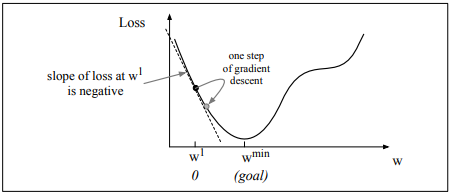
\includegraphics[scale=0.9]{gradstep.PNG}
		\caption{шаг градиентного спуска, для одномерных векторов черт}
		\label{fig:gradstep}
	\end{figure}
	
	По заданной случайной инициализации $w$ каким-то значением $w^1$ и предполагая, что функция потерь имеет форму, как на Рисунке~\ref{fig:gradstep}, требуется алгоритм, который сообщает, что на следующей итерации нужно сдвинуться влево или вправо, чтобы достичь минимума.
	
	Алгоритм градиентного спуска отвечает на этот вопрос, находя градиент функции потерь в данной точке и двигаясь в направлении, противоположном найденному.
	
	Величина движения в градиентном спуске - это наклон касательной $\frac{d}{dx}f(x;w)$, взвешенный скоростью обучения $\eta$. Большая скорость обучения означает, что нужно двигать $w$ больше на каждой итерации. Изменение параметра - это скорость обучения, умноженная на градиент:
	
	\begin{equation}
	w^{t+1} = w^t - \eta \dfrac{d}{dx} f(x;w)
	\end{equation}
	
	\subsection{Градиент для логистической регрессии}
	
	Для того, чтобы обновить веса, нужно ввести определение градиента. Для функции потерь кросс-энтропии:
	
	\begin{equation}
	L_{CE}(w, b) = -[y log \sigma(w \cdot x + b) + (1 - y) log(1 - \sigma(w \cdot x + b))]
	\end{equation}
	
	Возьмем производную:
	
	
	\begin{equation}
	\dfrac{\partial L_{CE}(w,b)}{\partial w_j} = [\sigma (w \cdot x + b) - y] x_j
	\end{equation}
	
	\subsection{Алгоритм стохастического градиентного спуска}
	
	Стохастический градиентный спуск - это online-алгоритм минимизации функции потерь, который вычисляет градиент после каждого обучающего примера и корректирует $theta$ (множество всех весов) \cite{19}.
	\\
	\noindent\fbox{%
		\parbox{\textwidth}{%
			\textbf{функция} Стохастический Градиентный Спуск ($L(), f(), x, y$) \textbf{возвращает} $\theta$ \\
			\text{ }\text{ } \# L - функция потерь \\
			\text{ }\text{ } \# f - функция, параметризированная $\theta$ \\
			\text{ }\text{ } \# x - вводы обучающей выборки \\
			\text{ }\text{ } \# y - выводы обучающей выборки (ярлыки) \\
			$\theta \leftarrow 0$ \\
			\textbf{Пока} требуется \\
			\text{ }\text{ } Для каждого прецедента ($x^{(i)}, y^{(i)}$) (в случайном порядке) \\
			\text{ }\text{ }\text{ }\text{ } 1. Вычислить $\hat{y}^{(i)}$ = $f(x^{(i)}; \theta)$ \\
			\text{ }\text{ }\text{ }\text{ } 2. Вычислить потерю $L(\hat{y}^{(i)}, y^{(i)})$ \\
			\text{ }\text{ }\text{ }\text{ } 3. $g \leftarrow \nabla_\theta L(f(x^{(i)}; \theta), y^{(i)})$ \\
			\text{ }\text{ }\text{ }\text{ } 4. $\theta \leftarrow \theta - \eta g$ \\
		}%
	}


	\begin{figure}[H]
		\caption{алгоритм стохастического градиентного спуска. Алгоритм может завершиться, когда сойдется, то есть, например, веса практически не изменяются.}
		\label{fig:gradalg}
	\end{figure}
	
	Параметр $\eta$ может быть скорректирован. Если он достаточно велик, то обучаемый будет делать слишком большие шаги, <<перепрыгивая>> минимум функции потерь, если слишком мал, то обучение будет занимаьт слишком много времени. Очень часто скорость обучения делают большой, затем постепенно её уменьшают. Таким образом, $\eta$ становится функцией от номера итерации $k$.
	
	\subsection{Регуляризация}
	
	Есть проблема с обучением весов, которые заставляют модель идеально совпадать с обучающей выборкой. Если черта полностью определяет какой-то класс, потому что она встречается только у него, то её будет дан огромный вес. Веса черт будут пытаться идеально подстроиться под обучающую выборку, моделируя даже факторы шума, случайно скоррелировавшие с классом. Эта проблема называется \textit{переобучением}. Хорошая модель должна хорошо обобщать обучающую выборку к тестовой выборке. Переобученная модель будет иметь слабые показатели обобщения.
	
	Для избежания переобучения, \textit{регуляризация} $R(Q)$ добавляется к функции потерь.
	
	\begin{equation}
	\hat{\theta} = \underset{\theta}{argmax} \text{ } logP(y^{(i)} | x^{(i)}) - \alpha R(\theta)
	\end{equation}
	
	Регуляризация призвана <<наказывать>> модель за слишком большие веса. Таким образом, веса, которые соответствуют обучающей выборке идеально, но при этом используют веса с слишком большими значениями, будут наказаны больше, чем веса, которые соответствуют выборке чуть хуже, но зато имеют меньшие значения веса. 
	
	Есть два распространённых способа посчитать регуляризацию. \textit{L2-регуляризация} - это квадратичная функция весов. Норма L2, $||\theta||_2$ - такая же, как \textit{Евклидово расстояние} вектора $\theta$ от начала координат. Если $\theta$ состоит из $n$ векторов, то:
	
	\begin{equation}
	R(\theta) = ||\theta||_2^2 = \sum_{j=1}^{n} \theta_j^2
	\end{equation}
	
	Тогда функция потерь становится такой:
	
	\begin{equation}
	\hat{\theta} = \underset{\theta}{argmax} \text{ } logP(y^{(i)} | x^{(i)}) - \alpha \sum_{j=1}^{n} \theta_j^2
	\end{equation}
	
	\textit{L1-регуляризация} - линейная функция от значений весов, названная так по L1 норме $||W||_1$, сумме модулей величин весов, также известна как \textit{Манхэттенское расстояние}.
	
	\begin{equation}
	R(\theta) = ||\theta||_1 = \sum_{i=1}^n |\theta_j|
	\end{equation}   
	
	Подставленное в функцию потерь:
	
	\begin{equation}
	\hat{\theta} = \underset{\theta}{argmax} \text{ } logP(y^{(i)} | x^{(i)}) - \alpha \sum_{j=1}^{n} |\theta_j|
	\end{equation}
	
	L1 регуляризацию в статистике часто называют \textit{lasso regression}, L2 - \textit{ridge regression}. L2 предпочитает, чтобы в модели было много  маленьких весов, L1 предпочитает разреженные решения с большими весами, но множеством нулевых весов.
	
	
	\section{Векторные представления и семантики}
	
	Роль контекста важна в представлении слов. Слова, которые появляются в похожих контекстах чаще имеют похожий смысл. Эту связь называют $гипотезой распределения$ ($distributional hypothesis$). В этой главе будут представлены векторные семантики, которые основываются на этой лингвистической гипотезе, обучаются представлениям значений слов, которые названы \textit{эмбеддингами}, непосредственно из текстов. 
	
	
	\subsection{Векторные семантики}
	
	Идея векторных семантик заключается в том, чтобы представить слово в виде точки на многоразмерном пространстве семантик. Векторы для представления обычно называют \textit{эмбеддингами}. 
	
	
	\begin{figure}[H]
		\centering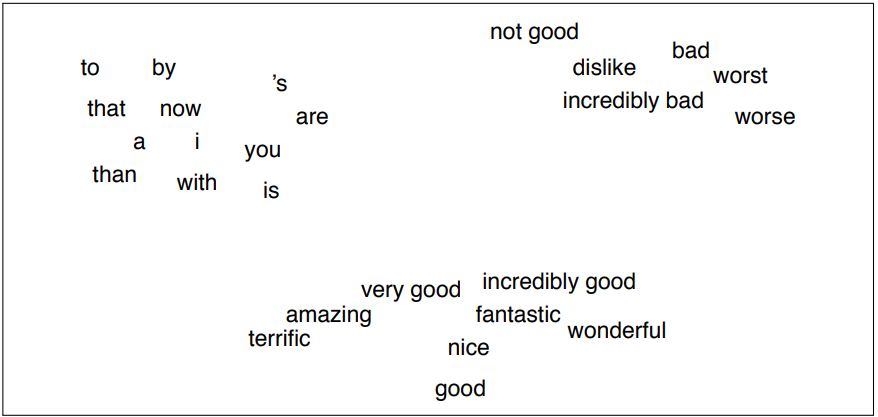
\includegraphics[scale=0.6]{sema.PNG}
		\caption{ двумерная проекция эмбеддингов некоторых слов и фраз, показывающая слова с похожими значениями рядом в пространстве.}
		\label{fig:sema}
	\end{figure}
	
	Можно заметить, что положительные и отрицательные слова расположены в разных частях рисунка.
	Векторные семантики очень полезны на практике тем, что они могут быть обучены автоматически из текста без каких-либо сложных обозначений или учителя.
	
	Векторные семантики являются стандартным способом представления слов в NLP.
	
	
	\subsection{Слова и векторы}
	
	Слова или модели распределения значений обычно основаны на \textit{матрице совмещения} (\textit{co-occurrence matrix}).
	
	Один из видов таких матриц - \textit{матрица терминов-документов}. Каждая строка обозначает слово в словаре, каждый столбец - документ, откуда слово было взято. Далее имет пример для четырёх пьес Шекспира.
	
	
	\begin{figure}[H]
		\centering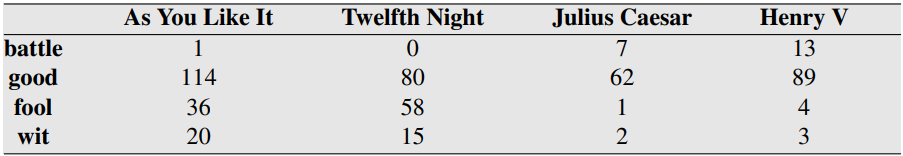
\includegraphics[scale=0.6]{shake.PNG}
		\caption{матрица терминов-документов для четырёх слов и четырёх пьес Шекспира}
		\label{fig:shake}
	\end{figure}
	
	Можно представлять вектор для документа как точка в |V|-мерном пространстве. Далее представлена проекция матрицы на  двумерную плоскость.
	
	\begin{figure}[H]
		\centering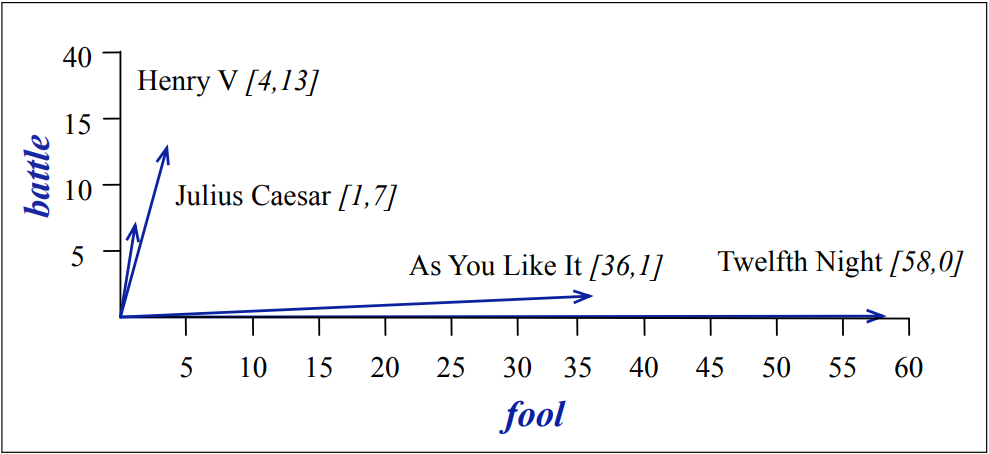
\includegraphics[scale=0.6]{proje.PNG}
		\caption{визуализация с измерениями, соответствующими словам \textit{battle} и \textit{fool}}
		\label{fig:proje}
	\end{figure}
	
	Матрица терминов-документов изначально была задуман для задачи информационного поиска, то есть, поиска документа $d$ из множества $D$ документов, который лучше всего подходит под запрос $q$.
	
	
	\subsection{Слова как векторы}
	
	Векторные семантики могут быть использованы для представления значения слов, ставя каждому слову в соответствие вектор.
	
	Вместо матрицы терминов-документов используются \textit{матрицы терминов-терминов}, чаще называемые \textit{матрицами слов-слов} или \textit{матрицами терминов-контекста} (\textit{term-term matrix}, \textit{word-word matrix}, \textit{term-context matrix}).
	 Это матрица размерности $|V| \times |V|$? каждая ячейка которой хранит количество раз слово в строке (целевое слово) и слово в столбце (контекст) встречались в каком-то контексте в одном корпусе.
	 
	 \subsection{Косинус для измерения расстояния между словами}
	 
	Для того, чтобы оценить похожесть двух целевых слов, нужна функция от двух слов, показывающая, насколько они близки по значению. Самая часто встречающаяся метрика - косинус угла между векторами.
	
	Косинус основан на скалярном произведении:
	
	\begin{equation}
	\textit{скалярное произведение} (v, w) = v \cdot w = \sum_{i=1}^{N}v_i w_i = v_1 w_1 + v_2 w_2 + \dots + v_N w_N
	\end{equation}
	
	В таком виде метрика имеет проблему: она предпочитает длинные вектора. Длина вектора определяется как:
	
	\begin{equation}
	|v| = \sqrt{\sum_{i=1}^N v_i^2}
	\end{equation}
	
	Самый простой способ модифицировать - это взять \textit{нормированное скалярное произведение}. 
	
	\begin{equation}
	a \cdot b = |a| |b| cos \theta
	\end{equation}
	
	\begin{equation}
	\dfrac{a \cdot b}{|a| |b|} = cos \theta
	\end{equation}
	
	Тогда расстояние между двумя словами может быть вычислено как:
	
	\begin{equation}
	cosine(v, w) = \dfrac{v \cdot w}{|v| |w|} = \dfrac{\sum_{i=1}^N v_i w_i}{\sqrt{\sum_{i=1}^N v_i^2}\sqrt{\sum_{i=1}^N w_i^2}}
	\end{equation}
	
	Иногда используют уже нормализованные векторы, то есть длины 1. Для нормализованных векторов косинус равен скалярному произведению.
	
	
	\subsection{TF-IDF: веса в терминах векторов}
	
	Частот в чистом виде недостаточно для того, чтобы оценить расстояние между словами. Одна из проблем заключается в том, что частоты сильно перекошены и недостаточно дискриминмативны. Возникает небольшой парадокс. Слова, которые появляются рядом друг с другом важнее, чем слова, которые появляются однажды или дважды. При этом слова, которые возникают достаточно часто (такие как \textit{хороший}, \textit{он}) на самом деле неважны. 
	
	Алгоритм \textit{tf-idf} - произведение двух множителей. 
	
	Первый - частота термина \cite{12}: количество раз слово $t$ встречается в документе $d$.
	
	\begin{equation}
	tf_{t,d} = count(t, d)
	\end{equation}
	
	Можно также взять $log_{10}$ он этого числа, так как если слово появляется в тексте 100 раз, это не значит, что оно в 100 раз более значимо для понимания документа.
	
	\begin{equation}
	tf_{t,d} = log_{10}(count(t, d) + 1)
	\end{equation}
	
	Второй множитель используется для того, чтобы дать вес словам, которые появляются в некоторых документах, так как такие слова полезны для их отделения. \textit{Частота документа} $df_t$ слова $t$ - это количество документов, в которых $t$ появляется. 
	
	\begin{equation}
	df_t = |D|, \forall d \in D: t \in d
	\end{equation}
	
	\textit{Обратная частота документа} $idf_t = N / df_i$, где $N$ - количество документов, используется для того, чтобы выделить дискриминативные слова.  
	
	\begin{equation}
	idf_t = \dfrac{N}{df_t}
	\end{equation}
	
	Следуя той же самой логике, что и с $tf_t$, возьмем $log_{10}$:
	
	\begin{equation}
	idf_t = log_{10} (\dfrac{N}{df_t})
	\end{equation}
	
	Вес слова $t$ в документе $d$ - произведение $tf_{t, d}$ на $idf_t$
	
	\begin{equation}
	w_{t, d} = tf_{t, d} \times idf_t
	\end{equation}
	
	\subsection{Word2vec}
	
	Здесь слова будут представлены как \textit{короткие} (длины 50-1000) и \textit{плотные} (большинство значений - не нули) векторами, так как плотные векторы работают в любой задаче NLP намного лучше, чем разреженные. Здесь будут представлен метод для очень плотных, коротких векторов, названный \textit{skipgram with negative sampling}, иногда его называют \textit{SGNS}. Алгоритм скипграмм - один из двух алгоритмов в пакете программного обеспечения, названном word2vec, поэтому сам алгоритм иногда называют также.
	
	Идея алгоритма заключается в том, что вместо того, чтобы считать как часто каждое слово $w$ встречается рядом с словом $w_1$, обучить бинарный классификатор, который будет отвечать, какова вероятность того, что $w$ окажется рядом с $w_1$.
	
	Революционной идеей является то, что можно использовать обрабатываемый текст как учителя для классификатора. Таким образом, не требуется собственноручно проставлять ярлыки.
	
	Word2vec \cite{20} хорош тем, что: во-первых, он упрощает задачу (бинарная классификация вместо предсказания слов), во-вторых, используется простая архитектура (обучается логистическая регрессия).
	
	Суть скипграмм в следующем:
	
	\begin{enumerate}
		\item Считать, что слово и его <<сосед>> - положительные примеры.
		\item Случайно выбрать другие слова из лексикона и считать их отрицательными примерами.
		\item Обучить логистическую регрессию на разделение этих классов
		\item Использовать веса регрессии как эмбеддинги. 
	\end{enumerate}
	
	
	
	
	\chapter{Специальная часть}
	
	
	
	
	\section{Содержательная постановка задачи}
	
	В настоящей научно-исследовательской работе ставится цель разработать систему выявления и мониторинга причин обращений клиентов банка на естественном языке, позволяющую получить причины на естественном языке. Под причиной в данной работе понимается часть исходного текста.
	
	Для достижения поставленной задачи необходимо решить следующие задачи:
	
	\begin{enumerate}
		\item Провести обзор и критический анализ соответствующих математических моделей, методов и алгоритмов, выявить их преимущества и недостатки, оценить границы применимости.
		
		\item Разработать математическое и алгоритмическое обеспечение системы, обеспечивающее корректную работу с русскоязычными текстами.
		
		\item Разработать программное обеспечение, реализующее основную функциональность на основе разработанного математического и алгоритмического обеспечения. 
		 
	\end{enumerate}
	
	\newpage
	
	\section{Математическая постановка задачи}
	
	Рассмотрим русскоязычный алфавит:
	
	\begin{equation}
	\Sigma = \{ \varepsilon_1, \dots, \varepsilon_{33}  \}
	\end{equation}
	
	Под словом длины $n$ будем понимать упорядоченный набор (вектор) букв алфавита $\Sigma$:
	
	\begin{equation}
	w = (\varepsilon_{k_1}, \dots, \varepsilon_{k_1}\varepsilon_{k_n}), k_1, \dots, k_n \in \{ 1, 2, \dots, 33\}
	\end{equation}
	
	Множество русскоязычных слов обозначим за $\Sigma^\ast$. При этом всякое упорядоченное подмножество слов будем называть текстом на русском языке, состоящем из $m$ слов.
	
	\begin{equation}
	W = \{w_1, \dots, w_m\} \subset \Sigma^\ast
	\end{equation}
	
	Обозначим время поступления обращения клиента за $t$.
	
	Запрос клиента -- кортеж из текста обращения и времени поступления.
	
	Обозначим множество причин как $R = W_r$ -- последовательность слов (эквивалентно тексту).
	
	Множество обращений - упорядоченная по неубыванию  времени поступления последовательность обращений клиентов:
	
	\begin{equation}
	Q = \{(W_1, t_1), \dots, (W_n, t_n)\}, t_i \leq t_{i+1}, \forall i \in [1, n-1]
	\end{equation} 
	
	На вход системы подается множество обращений.
	
	Необходимо разработать оператор $F$, который по заданному запросу построит вектор причин $R$.
	
	Также необходимо разработать оператор $F'$, который по заданному множеству обращений построит $R'$.
	
	
	\begin{equation}
	F(q) : 2^{\Sigma^\ast} \times \mathbb{R} \rightarrow 2^{\Sigma^\ast}
	\end{equation}  
	
	\begin{equation}
	F'(Q) : 2^{\Sigma^\ast} \times \mathbb{R} \times \mathbb{N} \rightarrow 2^{\Sigma^\ast}
	\end{equation}  
	
	\newpage
	
	\section{Функциональная схема решения}
	
	Структуру алгоритма нахождения корневых причин можно описать диаграммой, изображенной на рисунке~\ref{fig:scheme}.
	
	\begin{figure}[H]
		\centering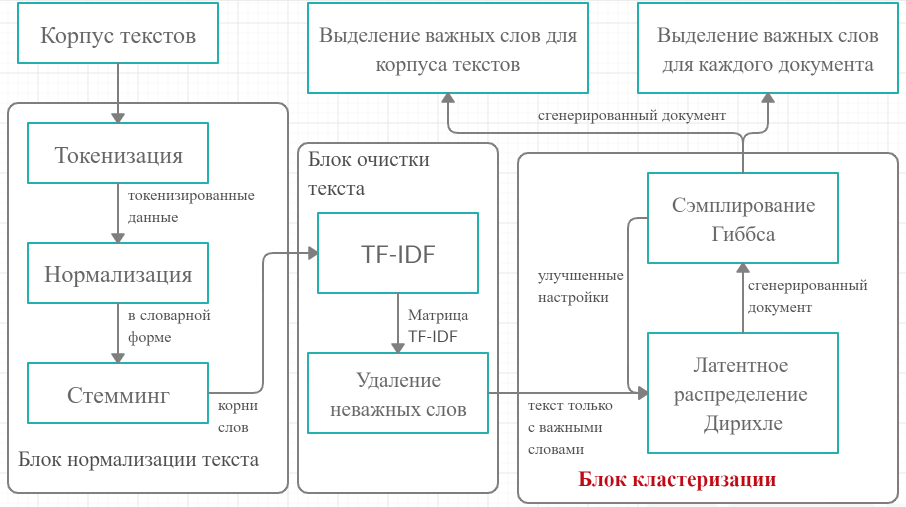
\includegraphics[scale=0.6]{SchemeFinal.PNG}
		\caption{Функциональная схема}
		\label{fig:scheme}
	\end{figure}
	
	\section{Описание предметной области}
	
	Данная работа основывается на том предположении, что все обращения клиентов разделяются на несколько больших тематик, связанных с банковской сферой:
	
	\begin{enumerate}
		\item Выпуск/перевыпуск/доставка карты. Здесь проблемы клиентов возникают с тем, что либо срок изготовления/перевыпуска/доставки карты был превышен, либо с тем, что в "личном кабинете" клиент видит, что карта готова к получению в банковском отделении, но по прибытию клиента оказывается, что карты на месте нет.
		
		\item Закрытие счета. В основном это запросы закрыть банковский счет в силу утери карты или утрате потребности в использовании этой карты.
		
		\item Отмена комиссии. Большинство сообщений о том, что клиент по ошибке пополнил счет "не той" карты, но при этом он не имеет возможности перевести на "ту" карты без комиссии. Поэтому он обращается в банк с просьбой это сделать.
		
		\item Эквайринг: оплата картой. Здесь встречаются сообщения о том, что при покупке какого-то товара деньги с карты были списаны, но на терминале этого отображено не было, следовательно, клиент заплатил, но не получил товар; он просит об отмене этой операции. 
		
		\item Другое. Это достаточно редкие случаи, связанные с банковскими продуктами. Например, из-за эпидемии COVID-19 много рейсов самолетов и поездов было отменено. Следовательно, начали поступали запросы о возвращении средств, потраченных на приобретение билетов на эти рейсы. Также часто это связано с обанкрочиванием фирм.
		
	\end{enumerate}
	
	\newpage
	
	\section{Формат входных и выходных данных}
	
	В настоящей работе в качестве источника входной информации для нахождения корневых причин служат данные Сбербанка, а именно сообщения клиентов в службу поддержки. Для понимания следует рассмотреть рисунок 16. Можно заметить, что в настоящее время такие задачи решает человек.
	
	
	\begin{figure}
		\centering
\includegraphics[scale=0.3]{input_data.jpg}
		\caption{Пример запроса клиента}
		\label{fig:input_data}
	\end{figure}
	
	То есть на вход поступают подобные тексты, неструктурированные, на естественном языке.
	
	Выводом системы будет множество слов и словосочетаний, характеризующих причину обращения клиента. Например, для рисунка~\ref{fig:input_data} система должна выдать подобный текст:
	
	\begin{center}
		\textbf{карта, не выпущена, перевыпустил, месяца}
	\end{center}
	
	
	По данному выводу легче понять, что обращение клиента поступило из-за просроченного периода перевыпуска карты.
	
	
	Также для всего множества текстов должен быть выдан подобный текст, отражающий общие тенденции запросов клиентов.
	
	
	
	\section{Разработанное алгоритмическое и математическое обеспечение}
	
	
	В данном решении используются следующие предположения:
	
	\begin{itemize}
		\item Предположение мешка слов, то есть того, что в тексте не важен порядок слов;
		\item Распределения "документ -- тема" и "тема -- слово" похожи на распределения Дирихле;
		\item слова, встречающиеся в большинстве документов, не важны для определения тематики, их обычно исключают из словаря и называют стоп-словами;
		\item слово в разных формах — это одно и то же слово;
	\end{itemize}
	
	\subsection{Модуль нормализации текста}
	
	Модуль нужен для первичной обработки сообщения, то есть для перевода его в вид, удобный для обработки следующими модулями. 
	
	На вход модулю поступает необработанное сообщение клиента, в том виде, в каком клиент его написал. То есть на вход модулю подается текст $W = \{w_1, w_2, \dots, w_m\}$
	
	Модуль состоит из четырех частей:
	\begin{enumerate}
		\item Токенизатор
		\item Нормализатор токенов
		\item Стеммер Портера
	\end{enumerate}
	
	Токенизатор соединяет слова, которые только вместе составляют смысловую единицу. В основном, речь идет об наименованиях (например, <<New York city>>), датах и организациях. 
	
	Для этого используется стандарт токенизации \textit{Penn Treebank} -- он выделяет клитики (то есть несамостоятельные слова, например, предлоги), объединяет слова, написанные через дефис, выделяет знаки препинания. Для непосредственной токенизации используется \textit{Python-based Natural Language Toolkit}, а точнее -- его функция  \textit{nltk.regexp tokenize}. После этого применяется алгоритм \textit{Byte Pair Encoding} для объединения наиболее часто встречающихся последовательностей токенов.
	
	Если рассмотреть с математической точки зрения, то токенизатор - это функция $T(W)$, которая в исходном тексте $W$ превращает $k$ наиболее часто встречающиеся последовательности из двух слов в новое слово.
	
	\begin{equation}
	W' = F(W)
	\end{equation}
	
	\begin{equation}
	w_{c_i}' = w_jw_{j+1}, order(w_jw_{j+1}) \leq k 
	\end{equation}
	
	Далее токенизированный текст поступает в нормализатор токенов, где все токены приводятся к нормальной (словарной) форме. Сначала производится \textit{Case folding} (\textit{Сжатие регистра}), это требуется для того, чтобы одни и те же слова, написанные в разных регистрах (например, слово, с которого начинается предложение), не считалось системой разными словами. 
	
	После этого к токенам применяется \textit{стеммер Портера}. Это детерминированный алгоритм, который последовательно <<отсекает>> от слова аффиксы. Этот алгоритм применяется для того, чтобы оставить от слов их стеммы, то есть корни, так как однокоренные слова очень часто близки по смыслу.
	
	Стеммированный текст передается на следующий модуль.
	
	
	
	\subsection{Модуль очистки текста}
	
	Входом этого модуля являются тексты, в которых сохранились только потенциально значимые слова. Для каждого элемента множества вычисляется его \textit{TF-IDF}. Эта метрика состоит из 2 множеителей: \textit{term frequency} и \textit{inverse document frequency}. Метрика устроена так, что она отдает предпочтение терминам, которые часто встречаются в данном документе и редко встречаются в других документах. Для более объективного результата оба множителя сглаживаются и логарифмируются, то есть:
	
	\begin{equation}
	tfidf(w) = \dfrac{log(tf+1)}{log(df+1)}
	\end{equation}
	
	После этого, слова, появляющиеся в корпусе 1 раз, а также слова, имеющие довольно большой TF-IDF удаляются, так как в большинстве случаев они являются неважными.
	
	
	\subsection{Модуль кластеризации}
	
	Для кластеризации текстов используется связка из Латентного распределения Дирихле и Сэмплирования Гиббса. 
	
	Латентное размещение Дирихле используется для того, чтобы сгенерировать документ, а Сэмплирование Гиббса - для того, чтобы улучшить распределение слов относительно топиков, после чего улучшенные данные о распределении слов относительно тем и топиков относительно слов поступают на вход Латентному распределению Дирихле.
	
	
	Общую схему Латентного размещения Дирихле можно увидеть на рисунке~\ref{fig:derihlet_scheme}.
	
	
	\begin{figure}[H]
		\centering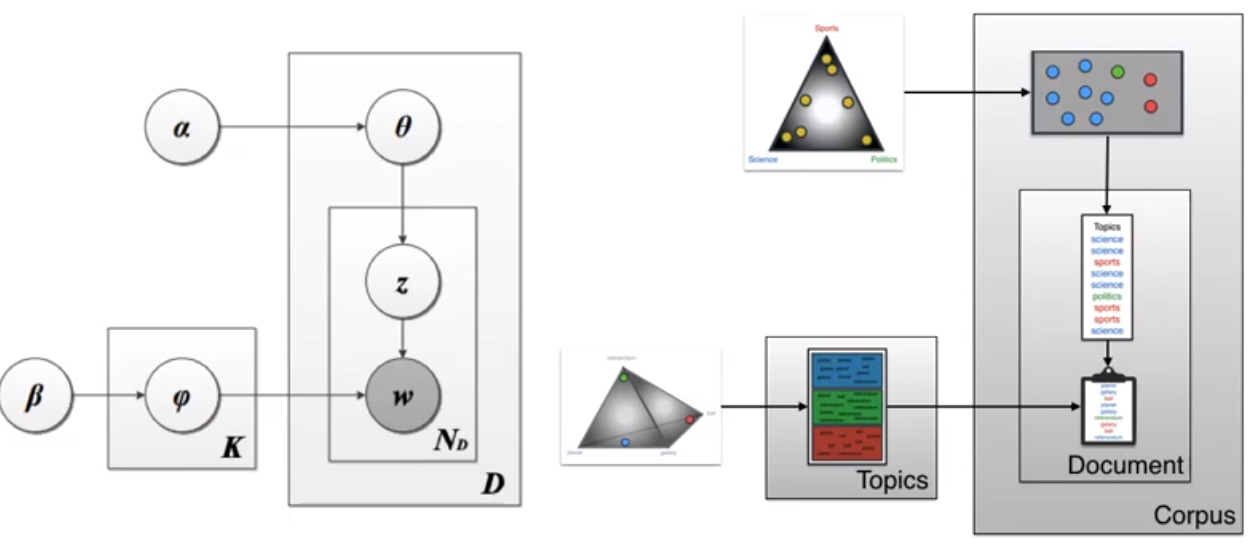
\includegraphics[scale=0.5]{derihlet_scheme.PNG}
		\caption{Общая схема латентного размещения Дирихле}
		\label{fig:derihlet_scheme}
	\end{figure}
	
	\begin{itemize}
		\item $ \alpha $ и $ \beta $ -- это коэффициенты распределений Дирихле.
		\item $ \theta $ -- мультиномиальное распределения для выбора топиков
		\item $ \phi_K $ -- несколько мультиномиальных распределений для выбора слов. 
		\item $z$ -- список топиков
		\item $z$ и $\phi_K$ объединяются, в результате получается $w$ -- список слов, являющийся сгенерированным документов.
		\item Данная процедура повторяется количество раз, равное количеству документов в корпусе.
 	\end{itemize}
	 
	 Сэмплирование Гиббса устроено следующим образом:
	 
	 Предположим, что документ принадлежит только одному топику, так как клиент делает обращение по одной конкретной проблеме.
	 
	 Тогда задача сводится к тому, чтобы отнести слова к топикам таким образом, чтобы документы, содержащие эти слова как можно сильнее относились к одному топику.
	 
	 Сначала случайным образом выбирается одно случайное слово из случайного документа. Далее для этого слова производится попытка отнести его к наиболее подходящей категории, предполагая, что остальные слова распределены правильно.
	 
	 Для каждой категории производится вычисление того, насколько слово подходит этой категории, по следующей формуле:
	 
	 \begin{equation}
	 	Topic_w := \underset{i}{argmax} \{(Cnt_{D_wT_i} + \varepsilon_1) \times (Cnt_{T_i} + \varepsilon_2)\}
	 \end{equation}
	
	где $Topic_w$ -- назначаемый слову $w$ топик, $Cnt_{D_wT_i}$ -- количество слов $w$ в документе, где находится слово $w$, относящиеся к топику $i$, $Cnt_{T_i}$ -- Количество слов $w$, относящихся к топику $i$ во всем корпусе. 
	
	Эта процедура повторяется $k$ раз, после чего предполагается, что все документы распределены по топикам правильно.
	
	\subsection{Вывод системы}
	
	Уже зная топик, к которому относится каждый документ а также зная для каждого слова, к какому топику оно относится, можно выдать слова, которые наиболее подходят для описания тематики документа. Для этого все слова, относящиеся к данной тематике сортируются в порядке встречаемости в документе, $n$ самых часто встречаемых подаются на выход. 
	
	Далее эта статистика суммируется, на ее основе $N$ самых часто встречаемых выводятся. Таким образом реализуется мониторинг.
	
	
	
	
	\chapter*{Заключение}
	\addcontentsline{toc}{chapter}{Заключение}
	
	В ходе выполнения работы были получены следующие результаты:
	
	\begin{enumerate}		
		\item Разработано программное обеспечение, позволяющее по корпусу текстов определить набор тематик для каждого документа, а также набор тематик для всего корпуса.	
		
		\item Программный модуль аппробирован на реальных данных обращений клиентов по банковским продуктам.
		
		\item Система реализована на языке программирования Python3, с использованием библиотек pandas, sklearn, numpy.
		
		\item Результаты опубликованы в сборнике тезисов 75-х Дней Науки НИТУ "МИСиС"
		
	\end{enumerate}
	
	
	
	
	\begin{thebibliography}{3}
		\bibitem{1}
		Фридл, Дж. Регулярные выражения = Mastering Regular Expressions. - СПб.: <<Питер>> , 2001. - 352 с. - (Библиотека программиста). - ISBN 5-318-00056-8.
		
		\bibitem{2}
		Lovins, Julie Beth. Development of a Stemming Algorithm // Mechanical Translation and Computational Linguistics. - 1968. - Т. 11.
		
		\bibitem{3}
		Маннинг К., Рагхаван П., Шютце Х. Введение в информационный поиск. - Вильямс, 2011. - 512 с. - ISBN 978-5-8459-1623-5.
		
		\bibitem{4}
		Crystal, David. A First Dictionary of Linguistics and Phonetics. Boulder, CO: Westview, 1980. Print.
		
		\bibitem{5}
		Ian H. Witten, Alistair Moffat, and Timothy C. Bell. Managing Gigabytes. New York: Van Nostrand Reinhold, 1994. ISBN 978-0-442-01863-4.
		
		\bibitem{6}
		P. Willett. The Porter stemming algorithm: then and now (англ.) // Program: Electronic Library and Information Systems. 2006. Vol. 40, iss. 3. P. 219223.  ISSN 0033-0337.
		
		\bibitem{7}
		В. И. Левенштейн. Двоичные коды с исправлением выпадений, вставок и замещений символов. Доклады Академий Наук СССР, 1965. 163.4:845-848.
		
		\bibitem{8}
		Jurafsky, D. and Martin, J.H. Speech and Language Processing: An Introduction to Natural Language Processing, Computational Linguistics, and Speech Recognition. Pearson Prentice Hall, 2009. 988 p. ISBN 9780131873216.
		
		\bibitem{9}
		Proceedings of the ITAT 2008, Information Technologies Applications and Theory, Hrebienok, Slovakia, pp. 23-26, September 2008. ISBN 978-80-969184-8-5
		
		\bibitem{13}
		Кельберт М. Я., Сухов Ю. М. Вероятность и статистика в примерах и задачах. Т. II: Марковские цепи как отправная точка теории случайных процессов и их приложения. -- М.: МЦНМО, 2010. -- 295 с. -- ISBN 978-5-94057-252-7.
		
		\bibitem{14}
		Domingos, Pedro \& Michael Pazzani (1997) <<On the optimality of the simple Bayesian classifier under zero-one loss>>. Machine Learning, 29:103-137. (also online at CiteSeer: [1])
		
		\bibitem{10}
		Bayes, T. (1763). An Essay Toward
		Solving a Problem in the Doctrine
		of Chances, Vol. 53. Reprinted in
		Facsimiles of Two Papers by Bayes,
		Hafner Publishing, 1963
		
		\bibitem{11}
		Mosteller, F. and Wallace, D. L.
		(1964). Inference and Disputed Authorship: The Federalist. SpringerVerlag. A second edition appeared in
		1984 as Applied Bayesian and Classical Inference.
		
		\bibitem{12}
		Luhn, H. P. (1957). A statistical approach to the mechanized encoding
		and searching of literary information.
		IBM Journal of Research and Development, 1(4), 309--317
		
		\bibitem{20}
		Mikolov T., Chen K., Corrado G., Dean J. Efficient Estimation of Word Representations in Vector Space // In Proceedings of Workshop at ICLR. -- 2013
		
		
		\bibitem{15}
		Geisser, Seymour (1993). Predictive Inference. New York, NY: Chapman and Hall. ISBN 978-0-412-03471-8.
		
		\bibitem{18}
		Tolles, Juliana; Meurer, William J (2016). "Logistic Regression Relating Patient Characteristics to Outcomes". JAMA. 316 (5): 533?4. doi:10.1001/jama.2016.7653. ISSN 0098-7484. OCLC 6823603312. PMID 27483067.
		
		
		\bibitem{16}
		Mitchell, Tom M. Machine Learning. -- WCB-McGraw-Hill, 1997. -- ISBN 0-07-042807-7.
		
		\bibitem{17}
		Акулич И. Л. Математическое программирование в примерах и задачах. -- М.: Высшая школа, 1986. ? С. 298-310.
		
		\bibitem{19}
		 Taddy, Matt (2019). "Stochastic Gradient Descent". Business Data Science: Combining Machine Learning and Economics to Optimize, Automate, and Accelerate Business Decisions. New York: McGraw-Hill. pp. 303?307. ISBN 978-1-260-45277-8.
		
		\bibitem{20}
		B. A. Frigyik, A. Kapila, and M. R. Gupta, “Introduction to the Dirichlet distribution and
		related processes,” UWEE, Tech. Rep. UWEETR-2010-0006, 2010.
		
		\bibitem{21}
		D. M. Blei, A. Y. Ng, and M. I. Jordan, “Latent Dirichlet allocation,” Journal of Machine
		Learning Research (JMLR), vol. 3, pp. 993–1022, 2003.
		
		\bibitem{22}
		Scott Deerwester, Susan T. Dumais, George W. Furnas, Thomas K. Landauer, Richard Harshman. Indexing by Latent Semantic Analysis // JASIS (41) 1990 pp. 391-407.
		
		
		
	\end{thebibliography}	
	%\chapter{список использованных источников}
	
	
\end{document}

